
% Preview source code

%% LyX 2.3.2 created this file.  For more info, see http://www.lyx.org/.
%% Do not edit unless you really know what you are doing.
\documentclass[oneside,english]{report}

\usepackage[T1]{fontenc}
\usepackage[utf8]{inputenc}
\usepackage{blindtext} 
\usepackage[english]{babel}
\setcounter{secnumdepth}{3}
\setcounter{tocdepth}{3}
\usepackage{amsmath}
\usepackage{amsthm}
\usepackage{float}
\usepackage{placeins}
\usepackage{listings}
\usepackage{esint}
\usepackage{pifont}% http://ctan.org/pkg/pifont
\newcommand{\cmark}{\ding{51}}%
\newcommand{\xmark}{\ding{55}}%


\makeatletter
%%%%% Examples of usages %%%%%
%\todo[inline,color=green!40]{Text} % add bubble comment
%\cite{liu2019wireless} %citation of AI-Wireless from bible.bib
%%%%%%%%%%%%%%%%%%%%%%%%%%%%%% LyX specific LaTeX commands.
\providecommand{\LyX}{L\kern-.1667em\lower.25em\hbox{Y}\kern-.125emX\@}

%%%%%%%%%%%%%%%%%%%%%%%%%%%%%% Textclass specific LaTeX commands.
\numberwithin{equation}{section}
\numberwithin{figure}{section}

%%%%%%%%%%%%%%%%%%%%%%%%%%%%%% User specified LaTeX commands.
\usepackage{pgfgantt}
%%% Gantt area %%%%
\definecolor{barblue}{RGB}{153,204,254}
\definecolor{groupblue}{RGB}{51,102,254}
\definecolor{linkred}{RGB}{165,0,33} 
%%% Gantaa ared END %%%%




\usepackage[linktoc=all]{hyperref}
\usepackage{xcolor}
\usepackage{pagecolor}
\usepackage{graphicx}
\usepackage{tocbibind}
\usepackage[colorinlistoftodos]{todonotes}
\usepackage{pdfpages}

\usepackage[
backend=biber,
style=alphabetic,
sorting=ynt
]{biblatex}
\addbibresource{bibli.bib}
\usepackage{csquotes}
\usepackage{lipsum}

\usepackage[ampersand]{easylist}
\usepackage[toc,section=chapter,acronym]{glossaries}
\usepackage[toc,page]{appendix}
\makeglossaries
\newglossaryentry{iot}
{
    name=IoT,
    description={Internet of Things}
}


\newglossaryentry{sdr}
{
    name=SDR,
    description={Software Defined Radio}
}


\newglossaryentry{rssi}
{
    name=RSSI,
    description={Received Signal Strength Indication}
}


\newglossaryentry{mimo}
{
    name=MIMO,
    description={Multiple Input Multiple Output}
}


\newglossaryentry{wifi}
{
    name=WiFi,
    description={Wirless Fidelity is a family of wireless networking technologies}
}

\newglossaryentry{rcs}
{
    name=RCS,
    description={Radar Cross Section}
}

\newglossaryentry{pdp}
{
    name=PDP,
    description={Power Delay Profile}
}
\newglossaryentry{rfic}
{
    name=RFIC,
    description={Radio-frequency integrated circuit}
}
\newglossaryentry{openbts}
{
    name=OpenBTS,
    description={Open \gls{bts} is a software-based \gls{gsm}}
}
\newglossaryentry{bts}
{
    name=BTS,
    description={Base transceiver station}
}
\newglossaryentry{gsm}
{
    name=GSM,
    description={Global System for Mobile Communications known as 2nd generation of the cellular}
}
\newglossaryentry{lte}
{
    name=LTE,
    description={ Long-Term Evolution known as 4th generation of the cellular}
}
\newglossaryentry{fpga}
{
    name=FPGA,
    description={Field-programmable gate array}
}
\newglossaryentry{pcb}
{
    name=PCB,
    description={Printed circuit board}
}
\newglossaryentry{usb}
{
    name=USB,
    description={Universal Serial Bus}
}
\newglossaryentry{80211ac}
{
    name=802.11ac,
    description={IEEE 802.11ac is a wireless networking standard in the 802.11 set of protocols}
}
\newglossaryentry{gnu}
{
    name=GNU,
    description={An extensive collection of free computer software licensed with \gls{gpl}}
}
\newglossaryentry{gpl}
{
    name=GPL,
    description={The \gls{gnu} General Public License}
}
\newglossaryentry{usrp}
{
    name=USRP,
    description={Universal Software Radio Peripheral}
}
\newacronym{emag}{EM}{Electromagnetic}

\newglossaryentry{rma}
{
    name=RMA,
    description={Range Migration Algorithm}
}
\newglossaryentry{gps}
{
    name=GPS,
    description={Global Positioning System}
}
\newglossaryentry{phy}
{
    name=PHY,
    description={Physical Layer}
}
\newacronym{ap}{AP}{Access Point}

\newglossaryentry{git_git}
{
    name=Git,
    description={Distributed version control}
}

\newacronym{itu}{ITU}{International Telecommunication Union}
\newacronym{ide}{IDE}{Integrated development environment}
\newacronym{poc}{PoC}{Proof of Concept}
\newacronym{rf}{RF}{Radio Frequency}
\newacronym{ssid}{SSID}{Service Set Identifier}

\newglossaryentry{UWB}
{
    name=UWB,
    description={Ultra Wide Band}
}


\newglossaryentry{EMI}
{
    name=EMI,
    description={Electromagnetic interference}
}
\newglossaryentry{wsn}
{
    name=WSN,
    description={Wireless Sensor Network}
}
\newacronym{cw}{CW}{Continues wave}
\newacronym{dc}{DC}{Direct current}
\makeatother

\begin{document}
%-TITLE PAGE-------------------------------------------------------------------------------
%	TITLE PAGE
%----------------------------------------------------------------------------------------

\begin{titlepage}

\newcommand{\HRule}{\rule{\linewidth}{0.5mm}} % Defines a new command for the horizontal lines, change thickness here

\center % Center everything on the page
 
%----------------------------------------------------------------------------------------
%	HEADING SECTIONS
%----------------------------------------------------------------------------------------

\includegraphics[width=7cm,height=7cm,keepaspectratio]{logo-new-round1.png}\\ % Include a department/university logo - this will require the graphicx package
\textsc{\Large School of Electrical \& Computer Engineering }\\[0.5cm] % Major heading such as course name
\qquad \qquad \quad 
\includegraphics[width=3cm,height=3cm,keepaspectratio]{logo_cse1.png}\\ % Include a department/university logo - this will require the graphicx package
\iffalse
\textsc{\large Communication Systems Engineering Program}\\[0.5cm] % Minor heading such as course title
\fi
%----------------------------------------------------------------------------------------
%	TITLE SECTION
%----------------------------------------------------------------------------------------

\HRule \\[0.4cm]
{ \huge \bfseries WiFi Based Wireless Imaging and Positioning for WSN
}\\[0.4cm] % Title of your document

 { \huge \bfseries 371-20-06}\\[0.4cm] % Title of your document
 \HRule \\[1.2cm]
%----------------------------------------------------------------------------------------
%	AUTHOR SECTION
%----------------------------------------------------------------------------------------

\begin{minipage}{0.4\textwidth}
\begin{flushleft} \large
\emph{Students:}\\
Mr. Oren \textsc{Zaharia} % Your name
\\
Mr. Efi \textsc{Dvir} % Your name
\end{flushleft}
\end{minipage}
~
\begin{minipage}{0.4\textwidth}
\begin{flushright} \large
\emph{Supervisor:} \\
Prof. Omer \textsc{Gurewitz} % Supervisor's Name
\end{flushright}
\end{minipage}\\[1cm]

% If you don't want a supervisor, uncomment the two lines below and remove the section above
%\Large \emph{Author:}\\
%John \textsc{Smith}\\[3cm] % Your name

%----------------------------------------------------------------------------------------
%	DATE SECTION
%----------------------------------------------------------------------------------------

{\large 31/08/2020}\\[0.5cm] % Date, change the \today to a set date if you want to be precise

%----------------------------------------------------------------------------------------
%	LOGO SECTION
%----------------------------------------------------------------------------------------


\includegraphics[width=3cm,height=3cm,keepaspectratio]{logo.png}\\[1cm] % Include a department/university logo - this will require the graphicx package
 
%----------------------------------------------------------------------------------------

\vfill % Fill the rest of the page with whitespace

\end{titlepage}

\iffalse
\pagestyle{empty} % No page numbers
\begin{titlepage}
Title
\definecolor{bgp}{RGB}{240,139,34}
\pagecolor{bgp} 
\end{titlepage}
\pagecolor{white} 
\fi

\chapter*{Preface}

\addcontentsline{toc}{chapter}{Preface}
\section*{Acknowledgements}
First and foremost we would like to express our deepest gratitude and appreciation to our supervisor, Prof. Omer Gurewitz. whom above of being our adroit guide in this academic endeavor is also our friend. With our utmost respect, we couldn’t have done it without you and your support. Thank you!
\newline
\newline
We would also like to thank the entire communication system engineering department teachers, staff and fellow students for a thrilling, incredibly hard yet satisfying 4 years of fun and adventure of a B.Sc diploma.
\newline
\newline
We would like to thank our families who supported us in every possible way. Your support allowed us to achieve such grate heights. 
\newline
\newline
We would also each like to thank one another for the true friendship and full commitment to the success of one another and this project. It's been a long ride, but every step was awesome. Thank you my friend!

Oren wants to thanks to Onyx, that gave him moments of Atnahta (break).
\begin{center}
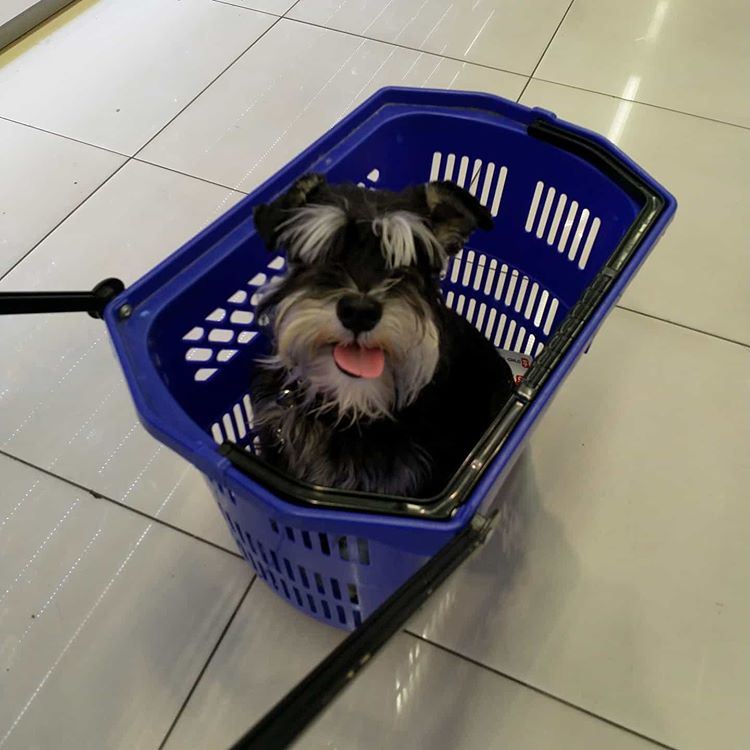
\includegraphics[scale=0.25]{figures/onyx_super.jpg}    
\end{center}



\section*{About us}

\addcontentsline{toc}{section}{About us}

 Mr. Oren Zaharia (28), a senior student of the Communication
Systems Engineering program at the Ben-Gurion University of The Negev, Israel. Graduated practical engineers in electrical and computer engineering with communication systems major. A 4 year 8200 alumni, experienced with \acrshort{rf} communication systems, signal engineering, and embedded programming.
Among his hobbies are: 
Programming, bicycling, hiking, soccer, Beitar Jerusalem, history, and more.
\newline
\newline
 Mr. Efi Dvir (30), a senior student of the Communication
Systems Engineering program at the Ben-Gurion University of The Negev, Israel. Graduated practical engineers in electrical and computer engineering with communication systems major. A 4.5 year 8200 alumni, experienced with \acrshort{rf} communication systems, signal engineering, and embedded programming.
Among his hobbies are: \gls{iot} sensors projects, painting, cooking, music, general craftsmanship, and more.
\newline
\newline
During their B.Sc studies, Mr. Efi Dvir and Mr. Oren Zaharia attended courses such as Signals and Systems, DSP, Wireless Networks Communication, and more.
\newline
\newline
Together, Mr. Efi Dvir and Mr. Oren Zaharia are brewing beer in their free time as well as sometimes enjoying a nice cold brew at the local pub.

\section*{About this report}

\addcontentsline{toc}{section}{About this report}

This report describes Mr. Efi Dvir's and Mr. Oren Zaharia's progress in their Communications
Systems Engineering program's final engineering project. Throughout this document, the reader might find references to articles and books who were used as an inspiration and technical basis to our project and are not Mr. Dvir and Mr. Zaharia's implementations. This report has been made using \LaTeX.

\section*{Intended audience}

\addcontentsline{toc}{section}{Intended audience}

The report is written for the academic community that want to review
and criticize our work or to be inspired or implement and learn our work.
The project in a range of final project implementations from simple
ideas implementations to complex ideas implementations. The report
assumed that the reader has some experience and knowledge in physics,
wireless sensors networks, radiofrequency, electrical wave propagation, and wireless communications. The report does not assume the experience of radar techniques, our tools, or any concrete knowledge in our implementation.

\section*{About this project}
This project is Mr. Efi Dvir's and Mr. Oren Zaharia's final engineering project as a partial requirement of the B.Sc  of Communications
Systems Engineering degree. This project suggests a method to infer knowledge of a sensor's surrounding environment using \gls{wifi} based wireless signals and their propagation properties. By using several methods to obtain information form \gls{wifi} signals this project strives to be able to classify the sensor's location and purpose (Temperature, pressure, humidity sensor which is located in a greenhouse in the backyard), in order to be able to use this information to configure the sensor as a part of a whole sensor information network. The project includes both a theoretical algorithmic view as well as practical hardware implementation using \gls{sdr}s. 
\addcontentsline{toc}{section}{About this project}




\renewcommand\contentsname{Table of Contents} 

\tableofcontents
\setcounter{tocdepth}{1} % fixing the problem of empty list of figures or tables

\listoffigures

\listoftables



\printglossaries



\chapter{Introduction}

\section{Background}

Smart environment is a relatively new concept, emerging in the early 1990s, where urban residents are interacting on a constant basis with informative objects, devices, sensors, and actuators to seamlessly better their lives. These collect information and process it in order to provide intelligent insights to the end-user and assist him in his daily routine. We treat a smart environment as an intelligent agent that perceives the state of the resident and the physical surroundings using sensors and acts on the environment using controllers in such a way that the specified performance measure is optimized \cite{Cook:2004:SET:1036248}.
Today, the number of sensors that monitor our environment is in persistent incline. With the entry of the Internet of Things (\gls{iot}) to the common household and workplaces, it is becoming more and more demanding for the user administrator to manage the rising number of sensors and actuators under his responsibility. The total installed base of \gls{iot} connected devices is projected to amount to 75.44 billion worldwide by 2025, a fivefold increase in ten years. The \gls{iot}, enabled by the already ubiquitous Internet technology, is the next major step in delivering the Internet’s promise of making the world a connected place \cite{iot_statista}.

\section{Motivation}

With each new sensor added to the sensor network, there is a need to configure its preferences and functions in order to comply with the network’s rules and order. Whereas a new sensor placed in its place usually needs to be manually configured with the information of its location and purpose. For example, when placing a smoke sensor in the kitchen, the sensor needs to be manually configured as the kitchen sensor in the user’s system monitoring the smoke levels above the stove. If this sensor has several abilities (besides smoke detection), each with its own data feed to the information system, it may be bothersome and tedious to deploy many of these data-gathering components of the network without some sort of automation. While exists some algorithms to organize the structure of the network’s traffic flow, there is a clear lack of methods to relieve the end-user of the task of configuring each sensor in its network manually.  
With our knowledge and passion for wireless communication, the thought of trying to engage the wireless capabilities, commonly found in many sensors, in order to assist in the configuration tasks of the user came to mind. By giving the sensor the ability to recognize and analyze its surroundings, a large amount of information could be gathered, organized, and used in order to help reach an assumption on what configuration profile may be best suited for a sensor. Thus, helping the user, or even relieving him entirely of the task of sensor configuration.

\section{Goals}
\paragraph{The Primary goal} of our project is to gather new side information about the structure and composition of the device’s environment using the propagation and reflection properties of wireless signals already in use in basic wireless devices. This information would be useful to assist in the classification of the room, the operations intended for the sensor, and general informative data that would better with the task of configuring the device’s function as part of the whole information network.
\paragraph{The Secondary goal} of our project is to use the gathered information to deduct insights regarding the composition of the device’s environment. By using machine learning tools and algorithms we would be able to classify the data that in turn will lead to the selection of a suitable configuration profile to set to the device itself. Thus, the gathered information will be used to configure the device in the user interface.
\section{Techniques}
\subsection*{}
There are several techniques in our disposal to obtain our primary goal:
\paragraph{Radio Frequency Imaging}
Using the transmission of wireless signals via \gls{mimo} antenna array in order to compose a 2D or 3D picture of the surroundings from the reflecting signals. By applying image recognition algorithms on the generated image, we would obtain environmental data to feed to the classifier.
\paragraph{Radar}
A detection system that uses radio waves to determine the range, angle, or velocity of objects. The range and angle of the device in relation to discovered objects in the vicinity would generate data. Each object discovered would carry a \gls{rcs} that will be used as environmental data and feed to the classifier.
\paragraph{Indoor Localization}
Using data from the communications protocols used by the device (\gls{rssi} for example in figure \ref{fig:rssi_triag_ex}), we would perform location triangulation survey in relation to known sources (\gls{wifi} routers for example). This location estimation would be feed to the classifier to classify in which room the device is located. We have already examine this option in our work-space at room 512/37 as seen in figure \ref{fig:rssi_triag_512}, where is exactly described in figure \ref{fig:rssi_triag_ex}, where each letter describes the anchor name.
\begin{figure}[H]
    \centering
    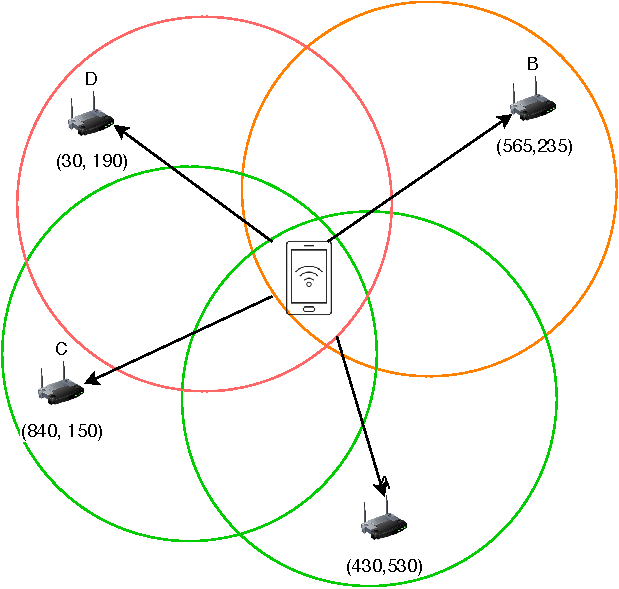
\includegraphics[width=5cm,height=5cm,keepaspectratio]{figures/rssi_triag.pdf}
    \caption{\gls{rssi} triangulation example}
    \label{fig:rssi_triag_ex}
\end{figure}
\paragraph{Radiation Holography}
Wireless data transmission systems such as \gls{wifi} or Bluetooth emit coherent light – electromagnetic waves with precisely known amplitude and phase. Propagating in space, this radiation forms  a hologram – a  two-dimensional wave-front encoding a  three-dimensional view  of all objects  traversed by the light beam \cite{Holl_2017}. Holographic data would be feed to the classifier to classify what are the objects in the room along to the room structure and size. Figure \ref{fig:holo_ex}  describes a holographic imaging process that generates 3D images using the microwave radiation of a \gls{wifi} transmitter experimented in  \cite{holography} "Holography of \gls{wifi} radiation". A space with a transmitter on the left and the resulting holographic images on the right.
\begin{figure}[H]
    \centering
    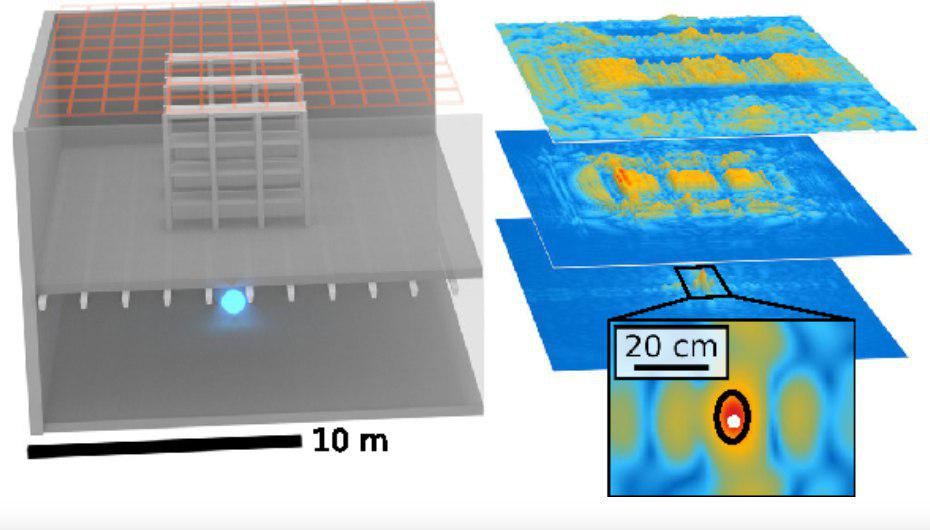
\includegraphics[width=5cm,height=5cm,keepaspectratio]{figures/fig_holg_ex.jpg}
    \caption{Holograph example}
    \label{fig:holo_ex}
\end{figure}
\paragraph{Power Delay Profile Decomposition}
The \gls{pdp} gives the intensity of a signal received through a multipath channel as a function of time delay. Each \gls{pdp} is unique and represents the channel time response.  By decomposing individual signal paths and using statistical analysis we would be able to generate data to feed to a learning machine. The figure \ref{fig:pdp_ex} gives an example to a power delay profile, where the axis time may be in nano-seconds or coarser, the power is in dB.
\begin{figure}[H]
    \centering
    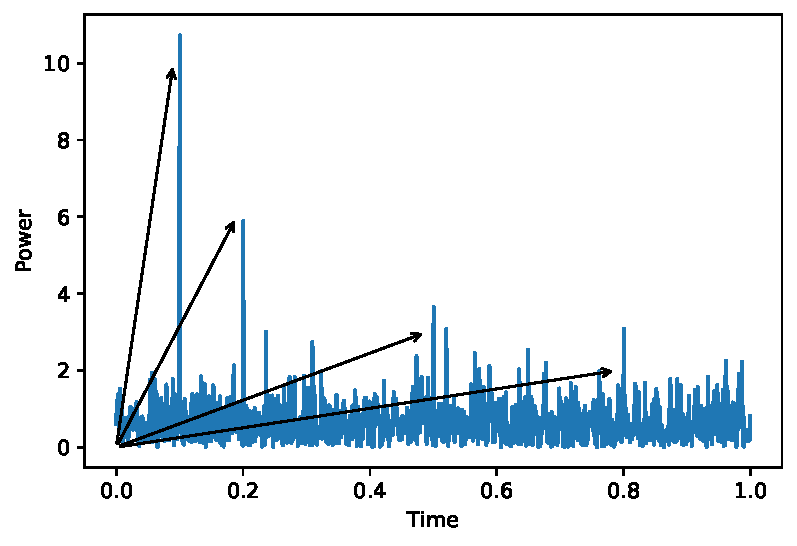
\includegraphics[height=7cm,height=5cm,keepaspectratio]{figures/pdp.pdf}
    \caption{\gls{pdp} example}
    \label{fig:pdp_ex}
\end{figure}
\subsection*{}


There are several techniques in our disposal to obtain our secondary goal:
\paragraph{Auto Encoders}an auto-encoder is a type of artificial neural network used to learn efficient data coding in an unsupervised manner \cite{wiki:xxx} By inputting general sampled signal data, we would obtain an output of data coding that in turn can be inputted into a classifier.
\paragraph{Machine learning}By using algorithms and statistical models that computer systems use to perform a specific task without using explicit instructions and by relying on patterns and inference instead, we would be able to infer properties that can assist in classifying the rooms and corresponding sensor configurations to suit it.
\paragraph{Neural networks}  - artificial neural networks may be used for predictive modeling, adaptive control and applications where they can be trained via a data-set. Self-learning resulting from experience can occur within networks, which can derive conclusions from a complex and seemingly unrelated set of information \cite{wiki:xxy}. By feeding the captured signals and information as a data-set to a pre-trained neural network we would derive conclusions regarding the device’s environment.
\chapter{The Project}
\section{Theory}

\subsection{Concepts}

In wireless radio communication, emitted signals experience a physical phenomenon known as multi-path propagation. A transmitted signal reaches the receiver after traveling by two or more paths. Walls and objects can reflect and scatter arriving signals as they cause changes in angle and time along the paths of the signal.
\paragraph{Mathematical Model \cite{wiki:multipath}}

The mathematical model of the multi-path can be presented using the
method of the impulse response used for studying linear systems.

Suppose you want to transmit a signal, ideal Dirac pulse of electromagnetic
power at time 0, i.e.

\begin{equation}
x\left(t\right)=\delta\left(t\right)    
\end{equation}

At the receiver, due to the presence of the multiple electromagnetic
paths, more than one pulse will be received, and each one of them
will arrive at different times. In fact, since the electromagnetic
signals travel at the speed of light, and since every path has a geometrical
length possibly different from that of the other ones, there are different
air traveling times (consider that, in free space, the light takes
$3\mu s$ to cross a $1km$ span). Thus, the received signal
will be expressed by (and seen in \ref{fig:multipath_ex})
\begin{equation}
y\left(t\right)=h\left(t\right)=\sum_{n-1}^{N-1}\rho_{n}e^{j\phi_{n}}\delta\left(t-\tau_{n}\right)
\end{equation}
where $N$ is the number of received impulses (equivalent to the number
of electromagnetic paths, and possibly very large), $\tau_{n}$ is
the time delay of the generic $n^{th}$ impulse, and $\rho_{n}e^{j\phi_{n}}$
represent the complex amplitude (i.e., magnitude and phase) of the
generic received pulse. Each pulse with its shift in time may be seen in figure \ref{fig:multipath_ex}. As a consequence, ${\displaystyle y\left(t\right)}$
also represents the impulse response function $h\left(t\right)$ of
the equivalent multi-path model.


\begin{figure}[h]
\centering
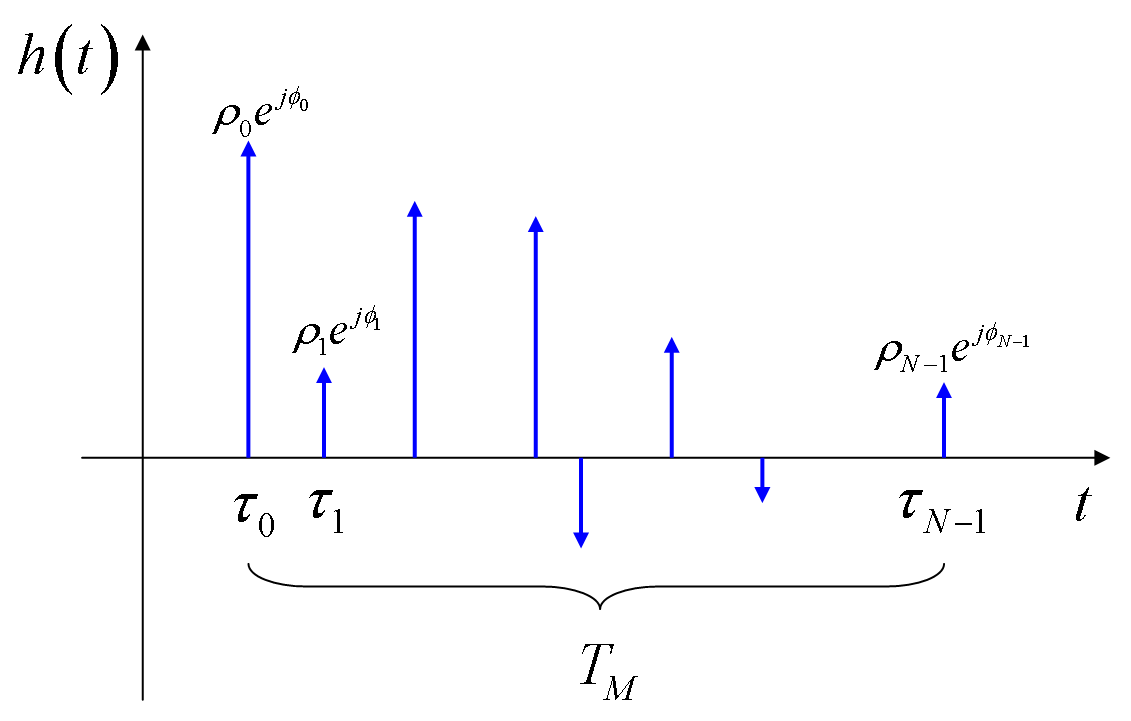
\includegraphics[width=7cm,height=7cm,keepaspectratio]{figures/Multipath_impulse_response.png}
\caption{Multi-path impulse response}
\label{fig:multipath_ex}
\end{figure}
The multi-path phenomena are always present in wireless communication, especially in indoor environments. It has been a long time that we consider multi-paths as interferences, noise, or simply nuisance. Profiles of multi-paths changes from location to location, thus, multi-path channel profile works as a unique and location-specific signature. Thus, instead of being considered as a nuisance, one can design various types of analytics based on the uniqueness of the multi-path channel state information. By fully exploiting the rich multi-path information, technology can decipher the propagation environment, revealing information that is usually disregarded. Such a technology approach can enable many cutting-edge \gls{iot} applications.
\paragraph{}
The multi-path phenomena can be further exploited by using multiple-input
and multiple-output (\gls{mimo}) in the transmitting as well as in the receiving
device.

In \gls{mimo} systems, a transmitter sends multiple streams by multiple
transmit antennas. The transmit streams go through a matrix channel
which consists of all $N_{r}$ paths between the $N_{t}$ transmit
antennas at the transmitter and $N_{r}$ receive antennas at the receiver.
Then, the receiver gets the received signal vectors by the multiple
receive antennas and decodes the received signal vectors into the
original information. A narrow-band flat fading \gls{mimo} system is modeled
as
\begin{equation}
y=Hx+n    
\end{equation}


where $y$ and $x$ are the receive and transmit vectors, respectively,
and $H$ and $n$ are the channel matrix and the noise vector, respectively \cite{wiki:mimo}.
\begin{figure}[H]
\centering
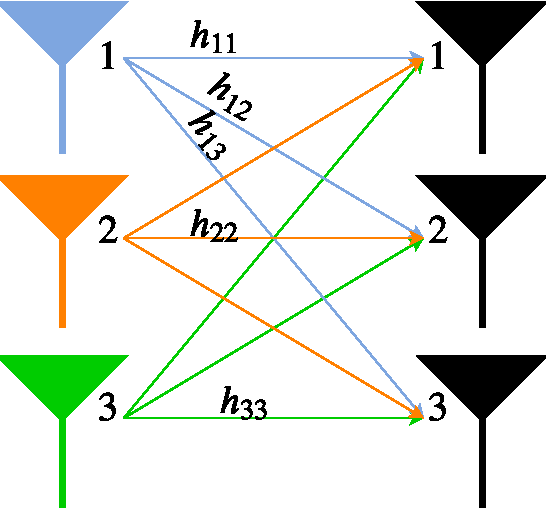
\includegraphics[width=7cm,height=7cm,keepaspectratio]{figures/MIMO_channel.pdf}
\caption{\gls{mimo} channel model}
\label{fig:mimo_channel_model}
\end{figure}
Each transmitting antenna (colored in blue orange and green in figure \ref{fig:mimo_channel_model}) is received differently in each receiving antenna (in the right side figure \ref{fig:mimo_channel_model}), thus, multiplying the amount of captured multi-path impulse responses. This expansion can further achieve unique spatial properties such as depth direction and other 3D information.
\todo{add radar concept, propagation concept, connect phase and distance}
\subsection{Techniques Survey}\label{Techniques Survey}

\paragraph{Radio Frequency Imaging}

is not a new technology, yet it has seen little commercial success
due to the cost and power consumption of a large number of antennas and radio transceivers
required to build such a system. Huang, Nandakumar, and Gollakota \cite{Huang:2014:FLW:2668332.2668344} describe the feasibility and limits of \gls{wifi} imaging by leveraging multi-path propagation. Their work introduces design and implementation which was able to identify objects inside a room (like a couch). Scott's thesis \cite{Scott:EECS-2017-191} introduces 3D microwave imaging for indoor environments which involves the use of antenna arrays, operating at microwave and millimeter-wave frequencies, for capturing images of real-world objects. His work focuses on using planar antenna arrays, operating between 17 and 26 GHz, to capture three-dimensional images of people and other objects inside a room. Scott suggests 3D microwave imaging algorithms for both dense and sparse antenna arrays as well as other algorithms such as colocated range migration algorithm \gls{rma} and a \gls{mimo} range migration algorithm which assist in the evaluation of the 3D space. Scott also suggests a design of antennas for microwave imaging and uses the Vivaldi tapered slot antenna in his implementations. 

\begin{figure}[h]
\centering
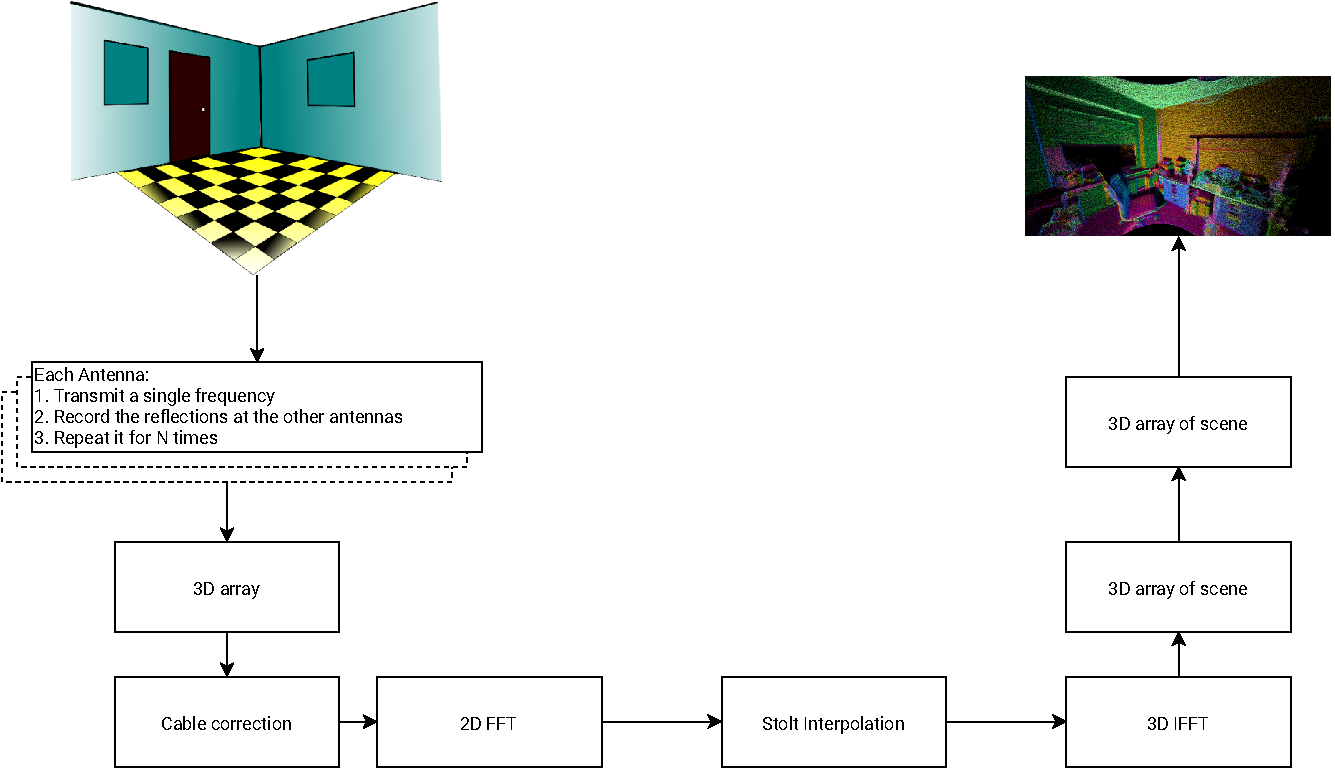
\includegraphics[width=12cm,height=7cm,keepaspectratio]{figures/RMA.pdf}
\caption{Block diagram for the colocated \gls{rma}}
\label{fig:rma_alg_ex}
\end{figure}

We intend to apply variations on Scott's work in order to comply with our hardware limitation and aspiration to use only popular protocols such as 2.4GHz  \gls{wifi} which is much lower and narrower than Scott's implementation. Yet, we need to obtain a lower resolution than Scott in order to apply room analysis processing on the data acquired. By trying to combine Huang, Nandakumar, and Gollakota's work with Scott's we would be able to achieve the collection of the information that we strive to obtain in order to be able to apply the inference of the surrounding environment. The algorithms described in figure \ref{fig:rma_alg_ex}, where each block is a part in the process from raw data that had been received in its $N$ antennas to the 3D array of the scene.

\paragraph{Indoor Localization} is a network of devices used to locate people or objects where \gls{gps} and other satellite technologies lack precision or fail entirely. Sen, Radunovic, Choudhury and Minka \cite{sen2012spot} explore the viability of precise indoor localization using physical layer information in \gls{wifi} systems. The algorithm they suggest demonstrates localization accuracies in the granularity of 1m x 1m boxes, called spots. They show through experiments that \gls{phy} layer channel information from existing \gls{wifi} deployments can be
an indicator of location. By synthesizing phase and time Lags and modeling the channel response they are able to apply clustering and classification algorithms which results in spot localization. 

\begin{figure}[h]
\centering
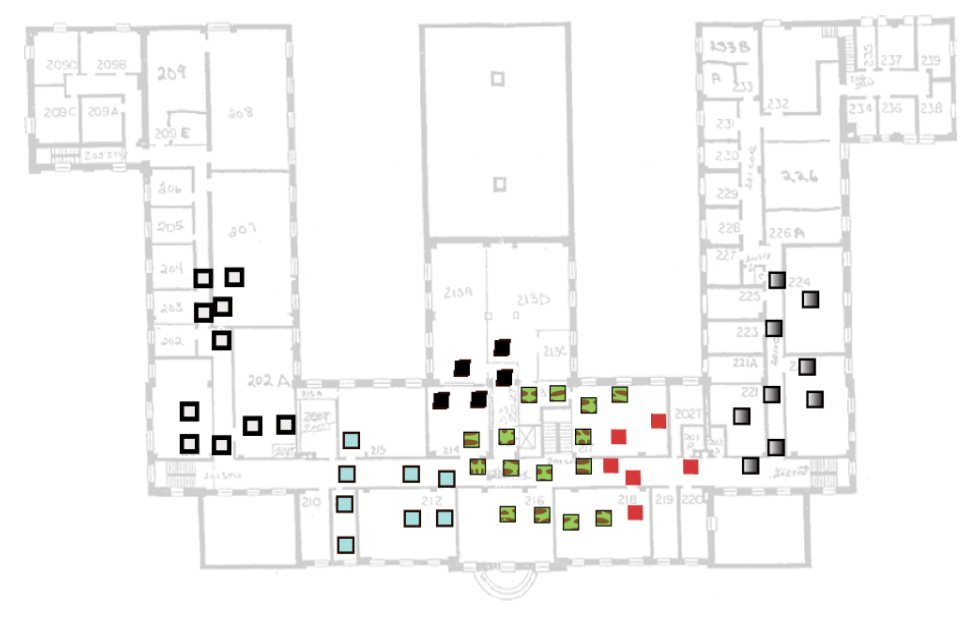
\includegraphics[width=8cm,height=7cm,keepaspectratio]{figures/spotloc.PNG}
\caption{Engineering building floor plan. Different sets of spots shown in different colors}
\label{fig:eng_bldg_floor_plan}
\end{figure}

Huang, Zheng, Xiao and Peng \cite{rssi} suggest localization based on the \gls{rssi} ranging Scope. In a \gls{rssi} based ranging algorithm, a node applies \gls{rssi} measurements to estimate its distances from the beacons, by using
a known signal propagation model. Such location information is only relative to the location of all connected \acrshort{ap}s in range. Thus, for exact localization, there is a need to know where the \gls{ap}s are located.
By combining \gls{rssi} localization and the \gls{phy} localization with other data obtained from other techniques we would be able to better analyze and infer information about the device's environment.
Figure \ref{fig:eng_bldg_floor_plan} shows different sets of spots located by indoor localization using \acrshort{ap}s positions.
\begin{figure}[H]
\centering
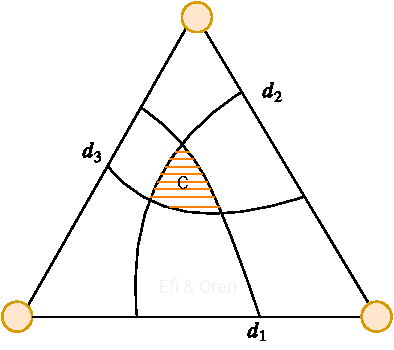
\includegraphics[width=6cm,height=6cm,keepaspectratio]{figures/rssi_regions.pdf}
\caption{Region division based on the \gls{rssi} value}
\label{fig:rssi_regions}
\end{figure}

\paragraph{Holography} is the science and practice of making holograms. Typically, a hologram is a photographic recording of a light field, rather than an image formed by a device without lens. \cite{wiki:holography}. In its pure form, holography requires the use of laser light for illuminating the subject and for viewing the finished hologram. Yet, Holl and Reinhard \cite{holography} demonstrate	a scheme	to	record	a	hologram	in	a	phase-coherent	fashion	 and	 recover	 three-dimensional	 views	 of	 objects	 and	 emitters	 and	 feeding	 the	 resulting	data	into	digital	reconstruction	algorithms.
Figure \ref{fig:holo_proc_ex}  describes a holographic imaging process that generates 3D images using the microwave radiation of a \gls{wifi} transmitter experimented in  \cite{holography} "Holography of \gls{wifi} radiation".
\begin{figure}[H]
\centering
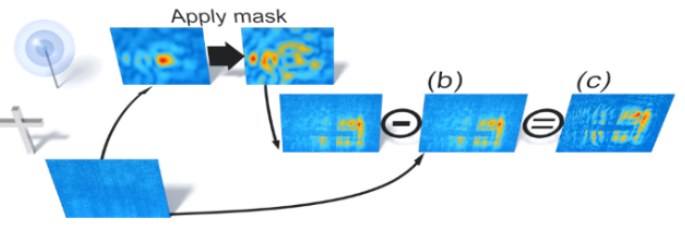
\includegraphics[width=10cm,height=6cm,keepaspectratio]{figures/holo.PNG}
\caption{Reconstruction	of objects using holography}
\label{fig:holo_proc_ex}
\end{figure}


\paragraph{Wireless Sensing} Embedded in wireless signals is information on an indoor environment that is captured during radio propagation, motivating the development of emerging wireless sensing technologies. Intelligent systems have become popular recently, in that with the help of learning they are capable of comprehending an object or even the world in the way humans do. For example, researchers have spent decades on computer vision or machine vision
systems that achieve a high-level understanding of digital images and videos that is comparable or even better than the human visual system. Can \gls{wifi} perceive an indoor environment? According to Liu and Wang\cite{liu2019wireless} the answer is yes. Applying statistical analysis on a data-set of captured signals is used for centimeter-accuracy indoor positioning and tracking, biometrics and vital signs estimation, motion and speed detection, and more. We intend to apply similar methods to the data-set of captured signals in order to create a sense of the device's environment. Many methods exist to apply indoor furniture and room recognition, Varvadoukas, Giannakidou, Gomez, and Mavridis \cite{Room_Recognition} use internet-derived models and object context to achieve this. While there are plenty of other methods to map and reconstruct the environment like 3D point clouds \cite{point_cloud} or set of 2D slices or just range measurements, they all rely on a data set we would obtain from the wireless sensor.

\newpage
\section{Block Diagram}
The following block diagram describes the inner goings of a sensor device in the stages taken to infer its surrounding environment using wireless-sensing.


\begin{figure}[H]
\centering
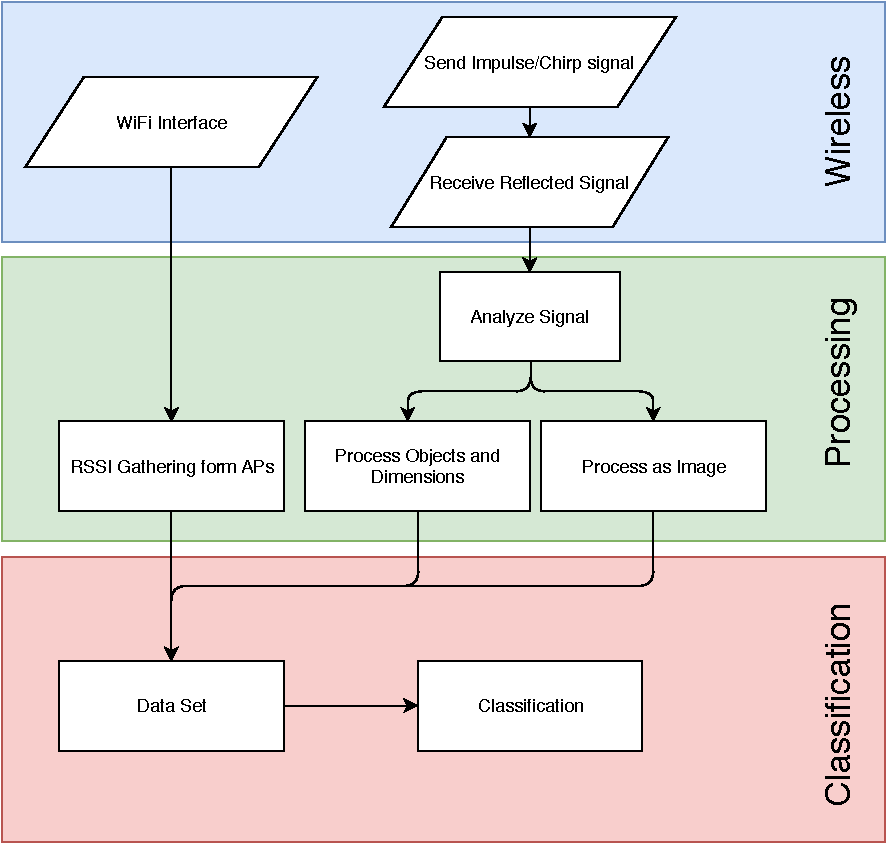
\includegraphics[width=12.5cm,height=20cm,keepaspectratio]{figures/block_diagram.pdf}
\caption{Block Diagram}
\label{fig:block_diagram_1}
\end{figure}




The Block Diagram (figure \ref{fig:block_diagram_1}) is divided in to three sections:
\begin{itemize}
    \item \textbf{Wireless Section} - The transmission and and reception of Ad-Hoc and standardized \gls{wifi} protocol signals.
    \item \textbf{Processing Section} - analyzing the received signals and processing them to an image or objects and dimensions. Creating data set from \gls{wifi} interface.
    \item \textbf{Classification} - Classifying space according to the combined created data sets.
    
\end{itemize}

\section{Practice}
\subsection{Constraints and solutions}
Out of the proposed techniques we choose to implement Radio Frequency Imaging and RSSI Indoor Localization wheres the Holography and Wireless Sensing techniques were found less suitable to be implemented under this project constraints.
\newline
The Holography technique which requires the illumination of a room using a radio signal and recording the received signals at another point in space required grate amount of mathematical development and exploration. In fact, this technique requires the solution of the well-known inverse problem \cite{wiki:Inverse_problem}. Since our problem is an inverse problem in the wave equations, it is very demanding in calculation taking all the wave scattering possibilities of the room along with the measurement system imperfections. Due to these reasons, this technique was forsaken under the scope of this project.
\newline
The Wireless Sensing techniques required us to apply statistical analysis on a data-set of captured signals, yet in order to do this, we first had to gather a data-set of signals. Due to the fact that one part of our project was dedicated to the creation of the radio system that would be used for our experiments we had a shortage of time to conduct many measurements so to create a sufficient data-set for this technique. Therefore, this technique was also forsaken under the scope of this project.
    

\subsection{Hardware}
\paragraph{Software-Defined-Radio}
In our project, we are using \gls{sdr} as our main hardware.
Software-defined radio (\gls{sdr}) is a radio communication system where components that have been traditionally implemented in hardware (e.g. mixers, filters, amplifiers, modulators/demodulators, detectors, etc.) are instead implemented by means of software on a personal computer or embedded system \cite{wiki:sdr}\cite[xxxiii]{book:139279}. While the concept of \gls{sdr} is not new, the rapidly evolving capabilities of digital electronics render practical many processes that were once only theoretically possible.
\paragraph{LimeSDR} is a low cost, open source, apps-enabled (more on that later) software defined radio (\gls{sdr}) platform that can be used to support just about any type of wireless communication standard.\cite{www:limesdr_brd}
\paragraph{Ettus \gls{usrp} B210} provides a fully integrated, single-board, Universal Software Radio Peripheral (\gls{usrp}™) platform with continuous frequency coverage from 70 MHz – 6 GHz. Designed for low-cost experimentation, it combines the AD9361 \gls{rfic} direct-conversion transceiver providing up to 56MHz of real-time bandwidth, an open and reprogrammable Spartan6 \gls{fpga}, and fast SuperSpeed USB 3.0 connectivity with convenient bus-power. Full support for the \gls{usrp} Hardware Driver™ (UHD) software allows you to immediately begin developing with \gls{gnu} Radio, prototype your own \gls{gsm} base station with \gls{openbts}, and seamless transition code from the \gls{usrp} B210 to higher performance, industry-ready \gls{usrp} platforms. An enclosure accessory kit is available to users of green \gls{pcb} devices (revision 6 or later) to assemble a protective steel case.\cite{www:ettus_b210}
\paragraph{Raspberry Pi} a series of small single-board computers. The last release of Raspberry Pi was in June 2019 with a 1.5GHz 64-bit quad core \href{https://en.wikipedia.org/wiki/ARM_Cortex-A72}{ARM Cortex-A72} processor. The board includes two \gls{usb} 3.0 ports and support \gls{80211ac} \gls{wifi}.
\subsection{Programs}
\paragraph{\gls{gnu} Radio}\gls{gnu} Radio is a free \& open-source software development toolkit that provides signal processing blocks to implement software radios. It can be used with readily-available low-cost external \acrshort{rf} hardware to create software-defined radios, or without hardware in a simulation-like environment. It is widely used in research, industry, academia, government, and hobbyist environments to support both wireless communications research and real-world radio systems \cite{www:gnuradio_about}.
The toolkit that is provided under \gls{gnu} Radio is written with C/C++ and Python. The libraries that are being used with are \href{https://www.boost.org/}{Boost} for C++ and \href{https://numpy.org/}{NumPy} that used \href{https://www.boost.org/}{Boost} and compiled under C/C++ to be used with Python.
\paragraph{CST Studio} a high-performance 3D \acrshort{emag} analysis software package for designing, analyzing and optimizing \acrshort{emag} components and systems.
\subsection{Work-space}
\paragraph{\href{https://www.overleaf.com}{Overleaf}} is an online \LaTeX{} editor that allows real-time collaboration and online compiling of projects to PDF format.
Overleaf is a freely-hosted and allows:
\begin{itemize}
    \item Track changes
    \item 2 collaborators per project
    \item Spell check
\end{itemize}
\paragraph{\href{https://github.com}{Github}} is a free cloud-based version software development  version control using \gls{git_git}.
\paragraph{\href{https://slack.com/}{Slack}} is a cloud-based that provides instant messaging platform. Slack offers features that goods for incollaboration projects.
\paragraph{\href{https://www.teamgantt.com/}{TeamGantt}} is a cloud-based gantt chart software can help plan your projects.
\paragraph{\href{https://www.jetbrains.com/}{JetBrains}} CLion and PyCharm that are and \acrshort{ide}s for C/C++ and Python respectively.

\paragraph{MicroPython}
MicroPython is a lean and efficient implementation of the Python 3 programming language that includes a small subset of the Python standard library and is optimized to run on microcontrollers and in constrained environments \cite{www:micro_python}.

\section{Simulation}

Before reaching our objective to create an image of a real scene. We need to have another step in our path, a simulation of a scene. A simulation is an action of pretending for the purpose of study, that is, by simulation we can study the algorithm, the effects of objects, mathematical theory and optimize the results of the proposed algorithm and method.


Because of the success of the simulations of the RF Imaging, we have put on hold and give up on the part of CST simulations which in retrospect would yield not too much for the RF Imaging which was our main goal.

\subsection{Radio Frequency Imaging Simulation}
To create a simulation we used a simple paint tool (similar to MS Paint of Microsoft), the output of the tool is a simple gray-scale bitmap, that is the created file is 2D-Matrix with values of 0 to 255. This file represents a delta size layer of XY in space. The simulator takes the created image file, and simulate the effect of transmitting a single Electromagnetic wave using an Isotropic antenna with a specific frequency, phase, and magnitude, the simulation calculates the reflected wave phase based on the time-delay of the image where the image is placed in known distance $z$.
Because that a better resolution of the file results in more computing time, the simulation is computing only values that are different from zero.
The simulation pretending to send a single electromagnetic wave, and calculate the reflection from all non-zero points in the bitmap file. The simulation generates a scene file that pretends to be a real measurement of a real scene that may be measured with an SDR or other RF equipment.
The generated scene file is characterized by a tensor of 3 dimensions where each entry in the tensor is a complex number that represents the magnitude and the phase of the reflections of the transmitted wave.

The following code integrate over the bitmap for dots that different from nil as given in Equation \ref{equ:reflection_sim}
\begin{equation}
    \sqint_{\text{Scene}}\exp\left(-j\cdot2\cdot k\sqrt{\left(x-x_{0}\right)^{2}+\left(y-y_{0}\right)^{2}+\left(z-z_{0}\right)^{2}}\right)
    \label{equ:reflection_sim}
\end{equation}
where $\left(x_0,y_0,z_0\right)$ represent the position of the transiting (and receiving) antenna and $\left(x,y,z\right)$ is the coordinate of point in the scene which has its own reflection. The integral is over all $\left(x,y,z\right)$ in space of the scene, in the simulation case $z$ is constant (one layer), $k$ is the wave-number $k = \frac{2\pi}{\lambda}$.
\newline
\begin{lstlisting}[language=Python,basicstyle=\scriptsize]
import numpy as np
def getIntegralDot2(img, k, _x, _y):
    args = np.argwhere(img)
    x_sc = img.shape[0]/Nx
    y_sc = img.shape[1]/Ny
    y = np.exp(-1j * 2* k * np.sqrt(0j +
                                    + np.power(args[:,0]*Dx/x_sc - _x, 2)
                                    + np.power(args[:,1]*Dy/y_sc - _y, 2)
                                    + np.power(Z1, 2)
                                   )
              )
    _img = img[args[:,0], args[:,1]]
    _img = _img.reshape(1, _img.shape[0])
    _img.shape
    return _img.dot(y)
\end{lstlisting}
The code is written in Python using NumPy package and implements Equation \ref{equ:reflection_sim}, see more in the appendices.
\begin{figure}[H]
    \centering
    
\includegraphics{figures/bgu3.png}
    \caption{Ben-Gurion Logo Bitmap}
    \label{fig:bitmap_bgu}
\end{figure}
Figure \ref{fig:bitmap_bgu} is the given input for the simulation, and its output is the input for the RMA algorithm.
\begin{figure}[H]
    \centering
    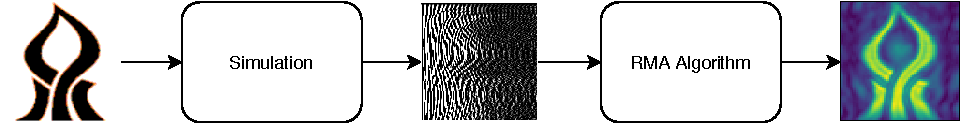
\includegraphics[scale=0.75]{figures/Simulation_Algo.pdf}
    \caption{Simulation Flow}
    \label{fig:simulation_flow}
\end{figure}

As may be seen in Figure \ref{fig:simulation_flow}, the input from Figure \ref{fig:bitmap_bgu} is used to generate a scene that is the input for the RMA algorithm that produced the "surprising" output.
\newline
\newline
One simulated 3D scene includes fully reflective points that are located in a spherical array formation. Each point in the scene space has a ray that is transmitted to, reflected, and received directly and each of these single rays experiences no path-loss. The reconstructed images of the scene, seen in \ref{fig:elipse}, shows the point array from two different perspectives (front and side views) wherein each perspective the Z-axis is summed to create a 2D image of reflective intensity.
\begin{figure}[H]
    \centering
    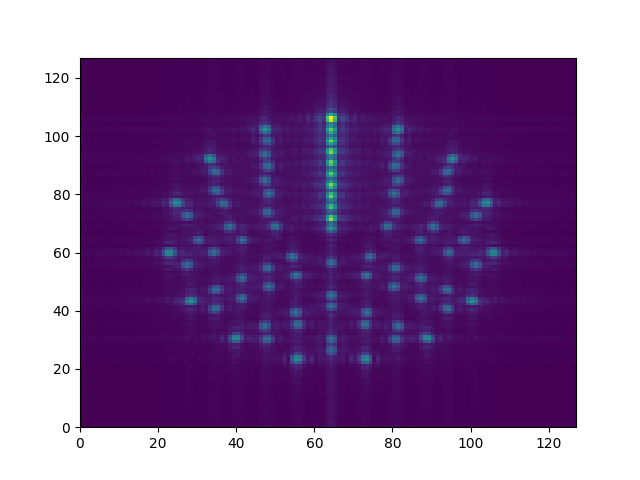
\includegraphics[scale=0.35]{figures/Elipse1.png}
    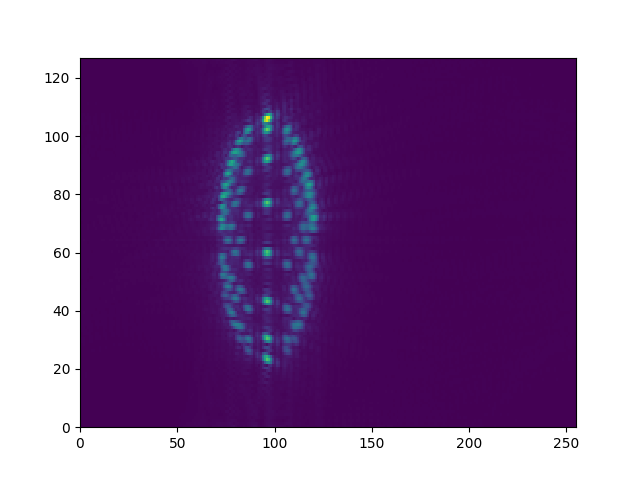
\includegraphics[scale=0.35]{figures/Elipse2.png}
    \caption{3D spherical array of fully reflective points scene results (Front and side view)}
    \label{fig:elipse}
\end{figure}

Following several other scene simulations, we decided to simulate the Ben-Gurion University logo as a flat object in the middle of the scene. The simulation is of 32X32 pixels summing the Z axis of the scene.
The results can be seen in \ref{fig:bgu_sim}.
\begin{figure}[H]
    \centering
    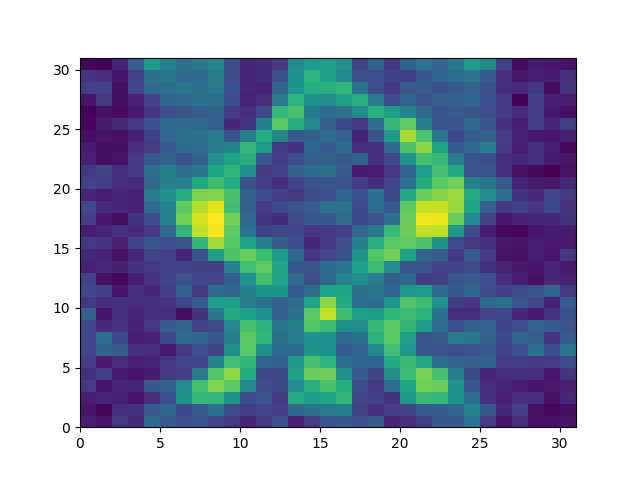
\includegraphics[width=6cm, height=8cm]{figures/Figure_1_bgu_323264.png}
    \caption{32X32 Reconstructed BGU logo}
    \label{fig:bgu_sim}
\end{figure}
\subsubsection{Resolution}

We noticed increasing the resolution of the simulation results in much better visual object recognition. The resolution of the reconstructed image correlates to the number of antennas in a sampling array. Thus, for better images, we pay with more samples and more processing of data resulting in the longer time needed to obtain an image.


\begin{figure}[H]
    \centering  
    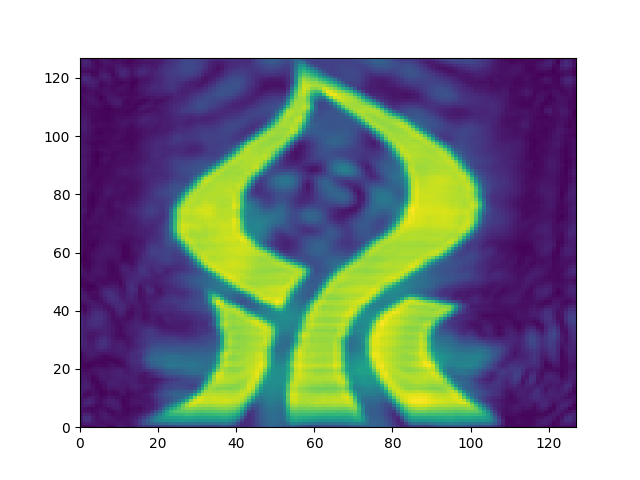
\includegraphics[trim=65 45 45 50,clip,width=3cm, height=4cm]{figures/Figure_bgu_128_128_64.png}
    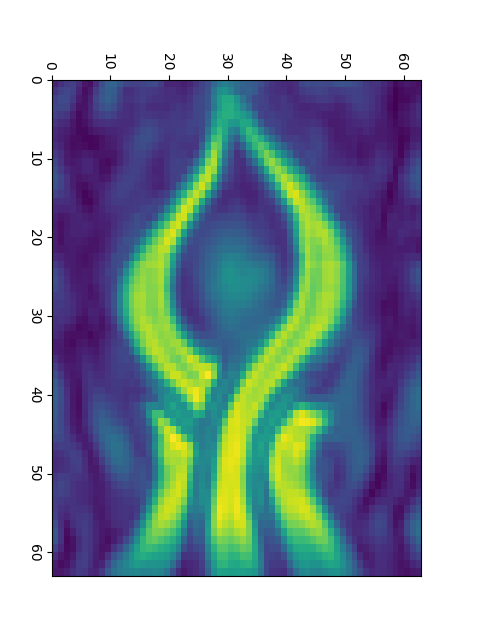
\includegraphics[trim=65 45 45 65,clip,width=3cm, height=4cm]{figures/Figure_1_bgu3.png}
    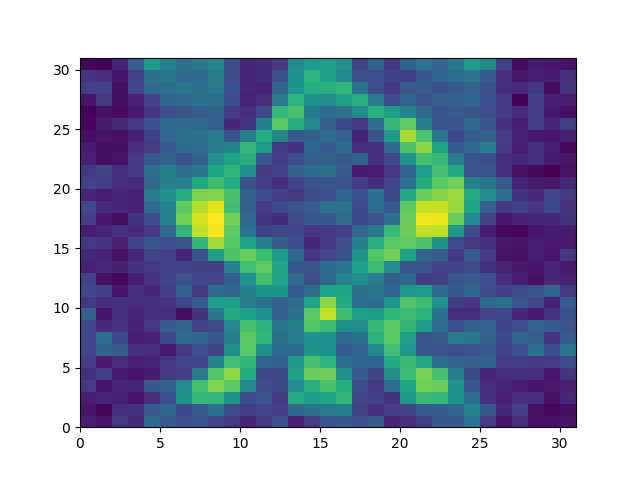
\includegraphics[trim=65 45 45 50,clip,width=3cm, height=4cm]{figures/Figure_1_bgu_323264.png}
  
    \caption{Reconstructed BGU logo: 32X32 positions (Right), 64X64 positions (Middle),128X128 positions(Left)}
    \label{fig:bgu_sim}
\end{figure}

\newpage
\section{Hardware setup}
In this project, we conducted implementations of the proposed methods. We created a hardware setup for each experiment that was needed to implement the method in use. The experiments can be divided into 2 objectives:
\begin{itemize}
    \item RSSI Triangulation 
    \item Radio Frequency Imaging
\end{itemize}


\subsubsection{RSSI Triangulation}
\label{rssi_hardware}
The required equipment for the experiments are:
\begin{enumerate}
\item \gls{wifi} enabled routers - Cisco-Linksys WRT54GS Wireless-G Broadband Router and others.
\item \gls{wifi} sensor node with packet parsing ability - 
Wemos D1 ESP8266 chip and ALPHA NETWORK 1 802.11b/g Long-Range Wireless USB Adaptor.
\end{enumerate}

We placed WRT54GS routers at random places in a room in order to use them as reference anchor points in space. 
\begin{figure}[H]
    \centering
    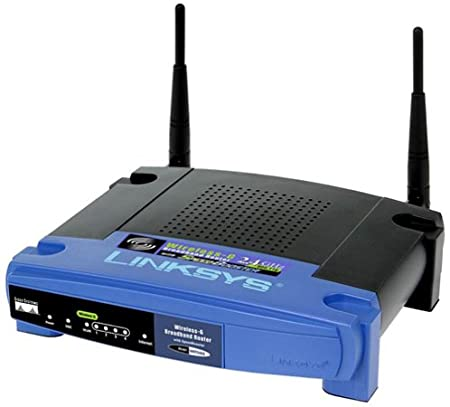
\includegraphics[scale=0.2]{figures/WirelessG.jpg}
    \label{fig:WirelessG}
    \caption{A WRT54GS 802.11b/g Router}
\end{figure}
 Each router was given a lexicographic letter (e.g A,B,C,D) as a \gls{ssid} to broadcast and it's location in the room was manually measured and recorded relative to an origin point $(0 m,0 m)$.
 \begin{figure}[H]
     \centering
     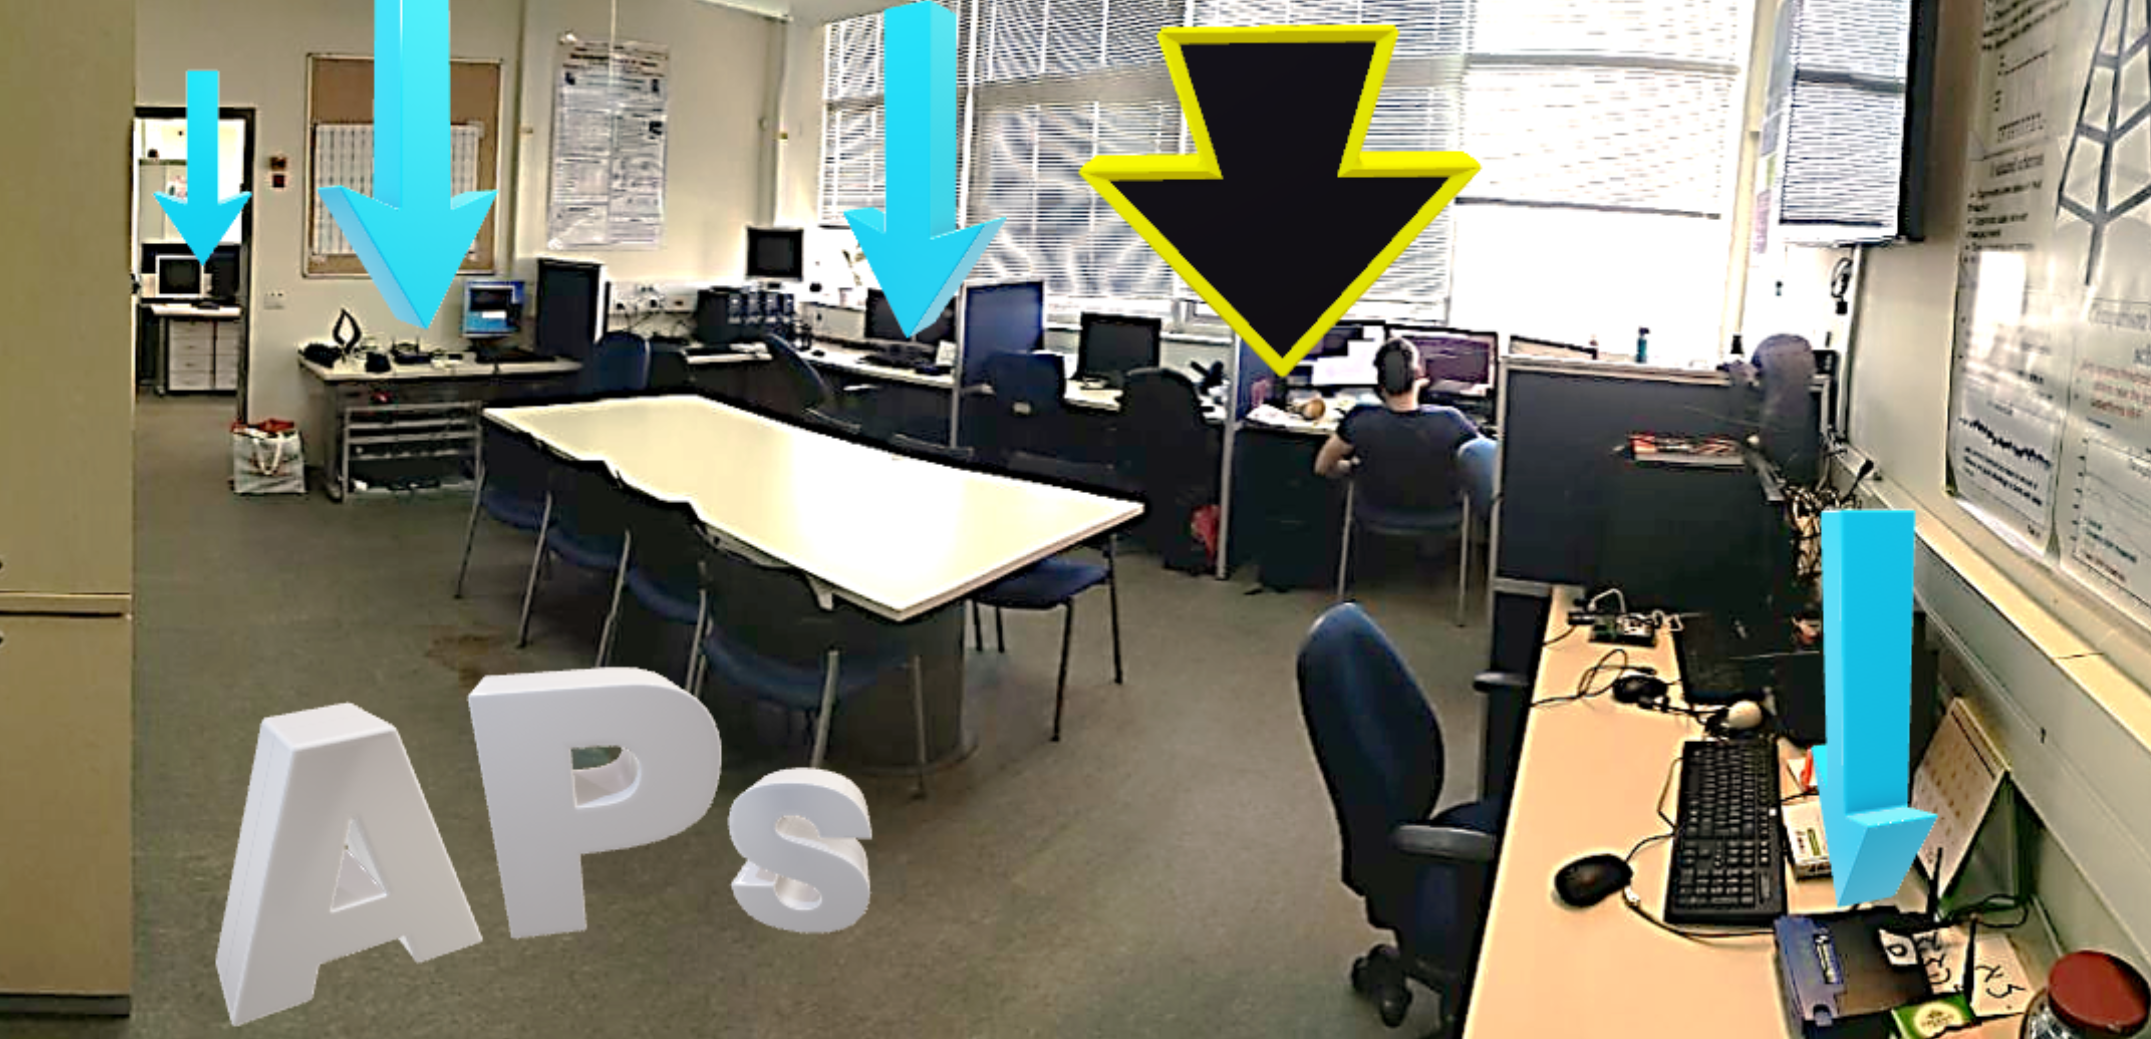
\includegraphics[scale=0.35]{figures/rssi_setup.png}
     \caption{\gls{ap}s (cyan) and sensor (black) setup in Lab 512}
     \label{fig:rssi_setup}
 \end{figure}
\subsubsection{Radio Frequency Imaging}
\label{rig}

The required equipment for the experiments are:
\begin{enumerate}
    \item Computer include USB3 GNU-Radio environment installed.
    \item SDR - In our experiments we have used B210 from Ettus.
    \item Automated XY grid positioning system - In our experiments we have used a 3D printer.
    \item A directional Vivaldi  RF transmit and receive antenna assembly with an RF shield between them to reduce co-channel interference (CCI) .
\end{enumerate}


\begin{figure}[H]
    \centering
    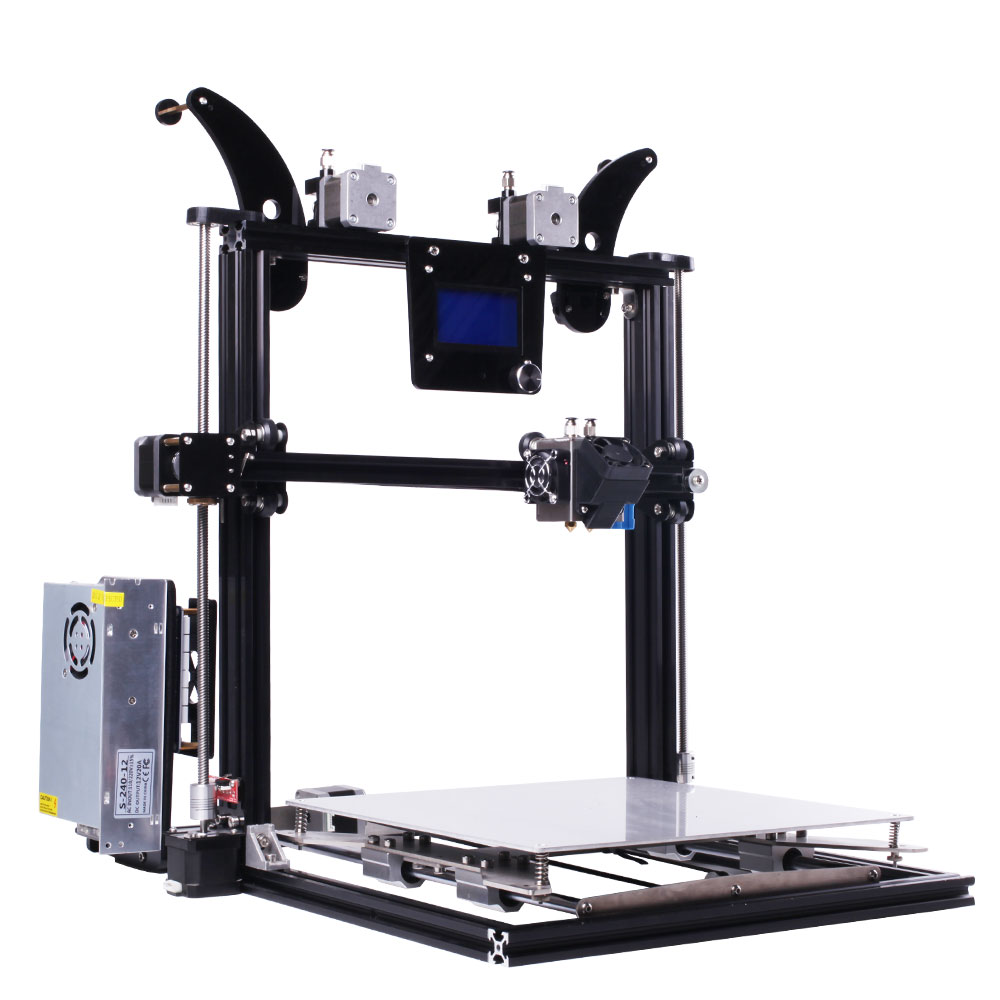
\includegraphics[scale=0.2]{figures/3d_Printer.jpg}
    
    \caption{The ZONESTAR 3D Printer}
    \label{fig:3d_Printer}
\end{figure}

In the following Figure \ref{fig:SAR_array}, the antenna assembly is mounted on top of the 3D printer moving head, instead of the filament heating element, such that the antenna assembly can move along X and Y axes. The computer is connected to the 3D printer engine controller using a USB cable and over a serial connection. The computer is also connected to the B210 SDR using USB3 and tunes the frequency of the SDR transmission and using it to receive the RF signals. The receiving and transmitting is base-band represented by a stream of 2-float numbers (complex), seen in Figure \ref{fig:SDR_IQ}. the received signal from the antenna is demodulated down to base-band and the down-converted signals are sampled into the I and Q (Real and Imaginary) representations of the sampled signal. 
\begin{figure}[H]
    \centering
    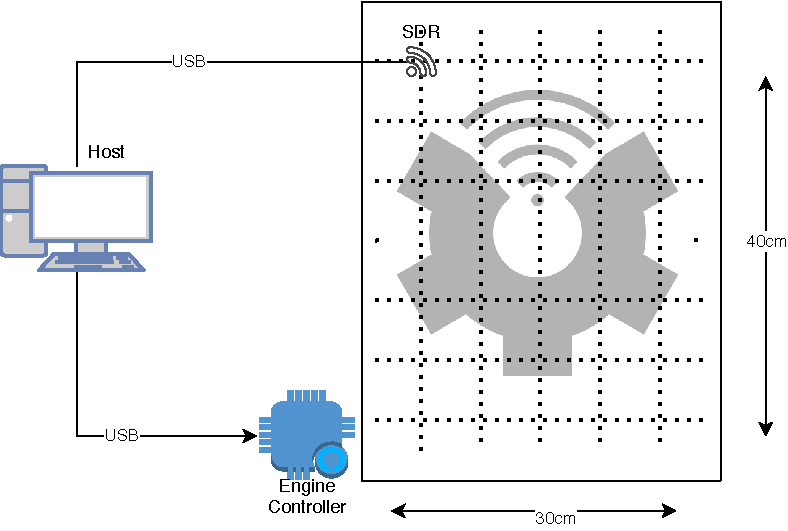
\includegraphics[scale=0.8]{figures/SAR_array.pdf}
    \caption{SAR Array Setup}
    \label{fig:SAR_array}
\end{figure}

It is very important to understand the need for synchronization of this part, lack of synchronization will result in wrong sampling and jitters and will add effects of a non-LTI system e.g. a non-causal system where the imaginary part from future samples combined with the present true part.
\newline
\newline
\begin{figure}[H]
    \centering
    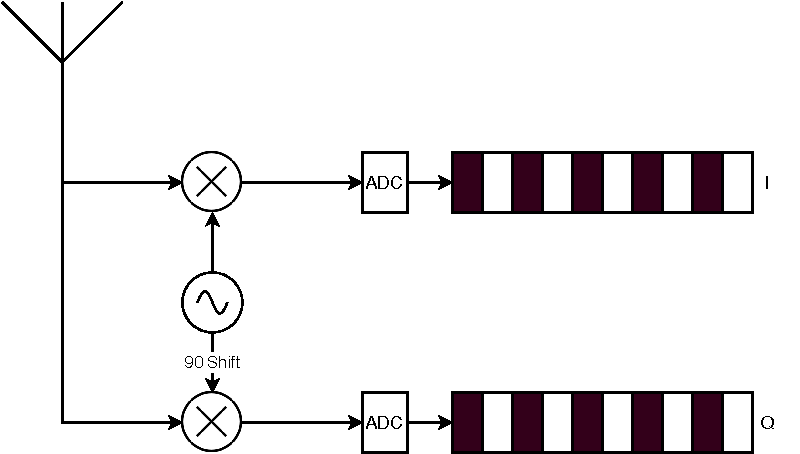
\includegraphics[scale=0.7]{figures/IQ.pdf}
    \caption{SDR sampling concept}
    \label{fig:SDR_IQ}
\end{figure}

The RF antenna assembly is composed of 2 Vivaldi antennas \cite{wiki:Vivaldi_antenna} which are a co-planar broadband-antenna, which is made from a solid piece of sheet metal, a printed circuit board, or from a dielectric plate metalized on one or both sides. This assembly is located on the head of the printer that can be seen in Figure \ref{fig:3d_Printer}, which is the 3D-Printer that we have used.

\begin{figure}[H]
    \centering
    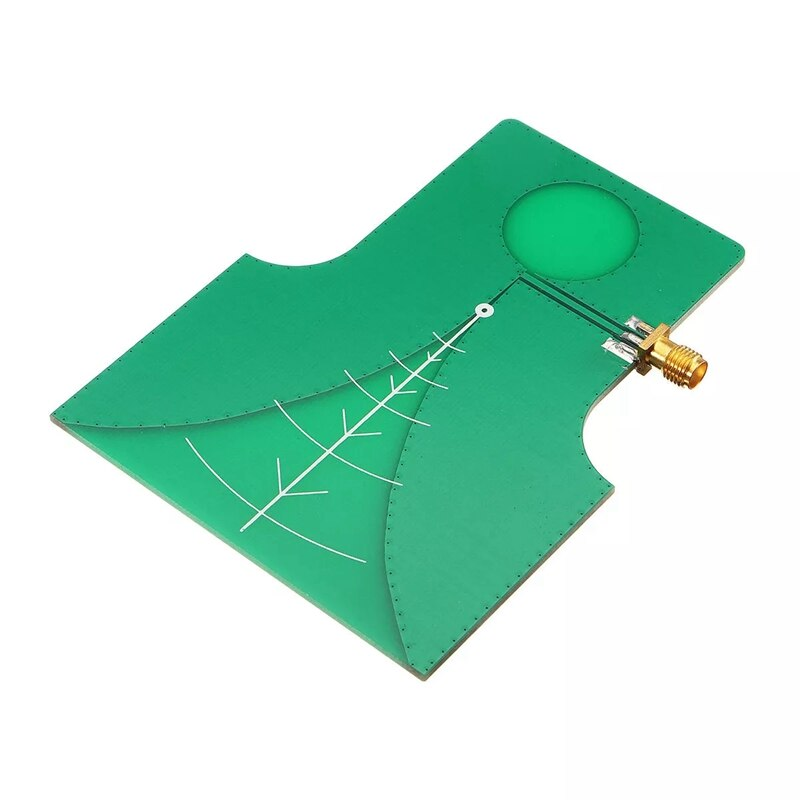
\includegraphics[scale=0.9]{figures/Vivaldi.jpg}
    \caption{Vivaldi antenna}
    \label{fig: Vivaldi antenna}
\end{figure}
The antenna we used, seen in \ref{fig: Vivaldi antenna}, is
a high gain directional wide-band antenna suitable for directional radio signal transmission and reception. Frequency range: $2.4 \text{GHz}-10.5 \text{GHz}$, linear polarization with a rated gain of $7 \text{dBi}$ and a return loss of $10 \text{dB}$.
We found this antenna to be most suitable for \gls{UWB} positioning, \gls{wifi} $2.4 \text{GHz}$ and $5.8 \text{GHz}$ and other common frequencies.
\newline
\newline
We placed the transmitting and receiving antennas in parallel to each other and with a $10 \text{cm}$ \acrshort{rf} \gls{EMI} shielding \cite{wiki:EMI_Shielding} in between.
\begin{figure}[H]
    \centering
    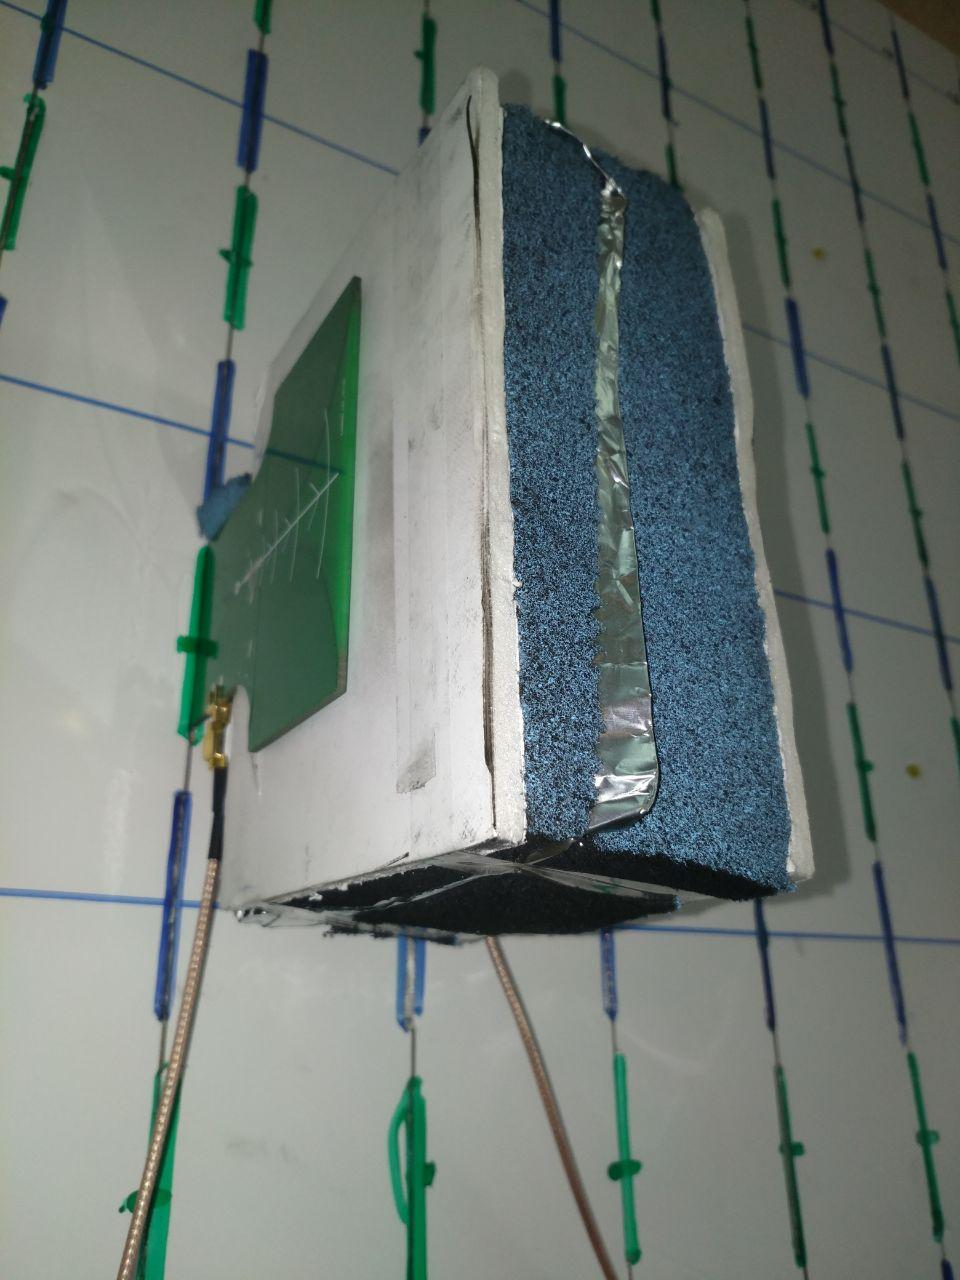
\includegraphics[scale=0.4]{figures/Antenna_assembly.jpg}
    \caption{Antenna assembly}
    \label{fig:Antenna assembly}
\end{figure}
The \gls{EMI} shielding purpose is to reduce the amount of energy picked up by the receiving antenna from the transmitting antenna at close range.  Meaning to reduce the signal sampled at a virtual minimal distance of $10 \text{cm}$ (the distance between the antennas). In order to further block the co-channel interference between the antennas we have placed an aluminum foil reflector in the middle of the \gls{rf} \gls{EMI} shielding. This shielding attenuation was tested and found to be greater than $10 \text{dB}$.
\newline
\newline
The antenna assembly was connected to the moving head of the 3D printer X,Y movement rig. The entire testing rig can be seen in \ref{fig:RF_Imaging_rig}.

\begin{figure}[H]
    \centering
    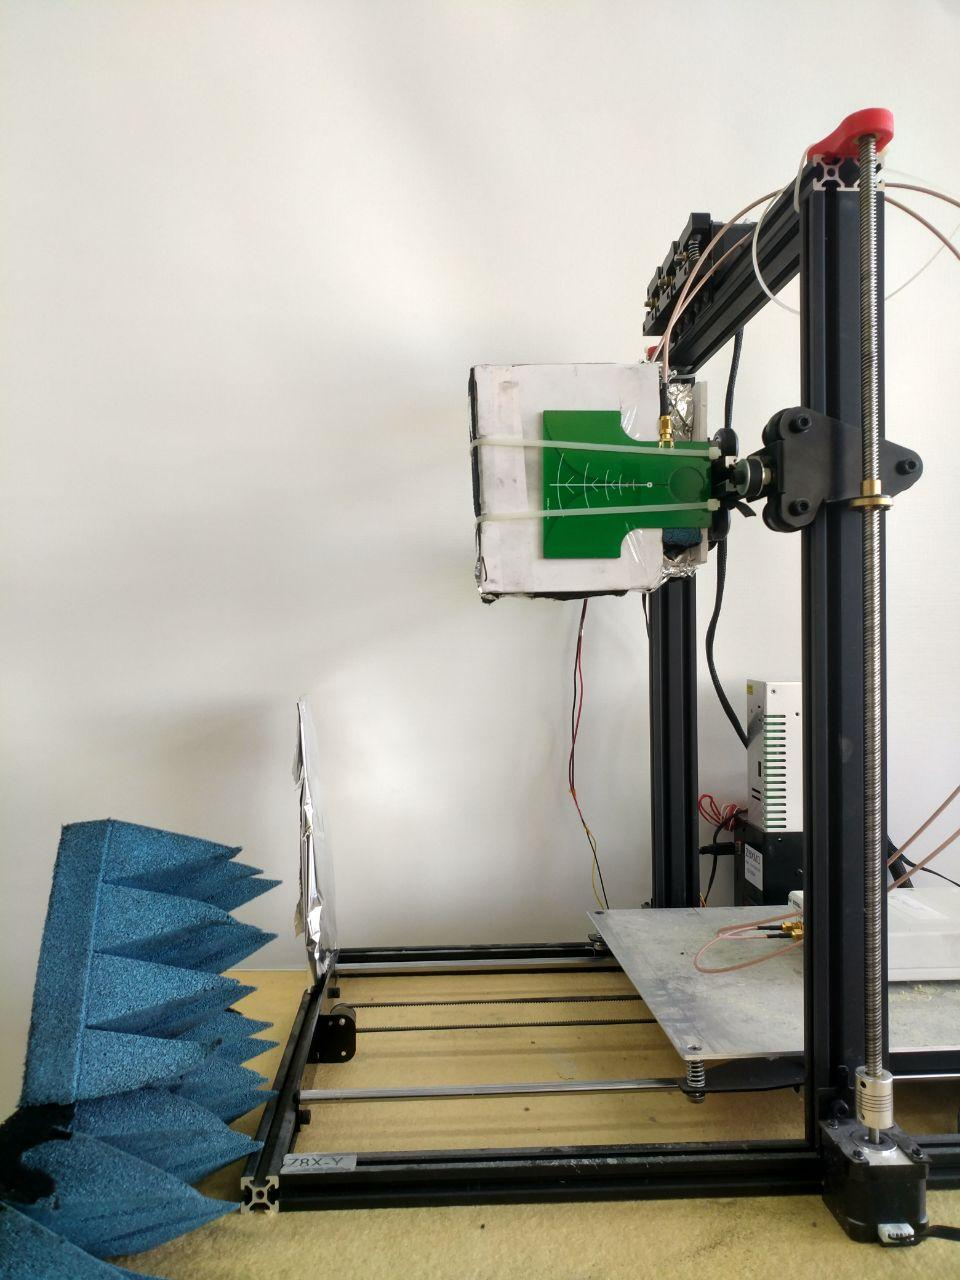
\includegraphics[scale=0.5]{figures/Rig.jpg}
    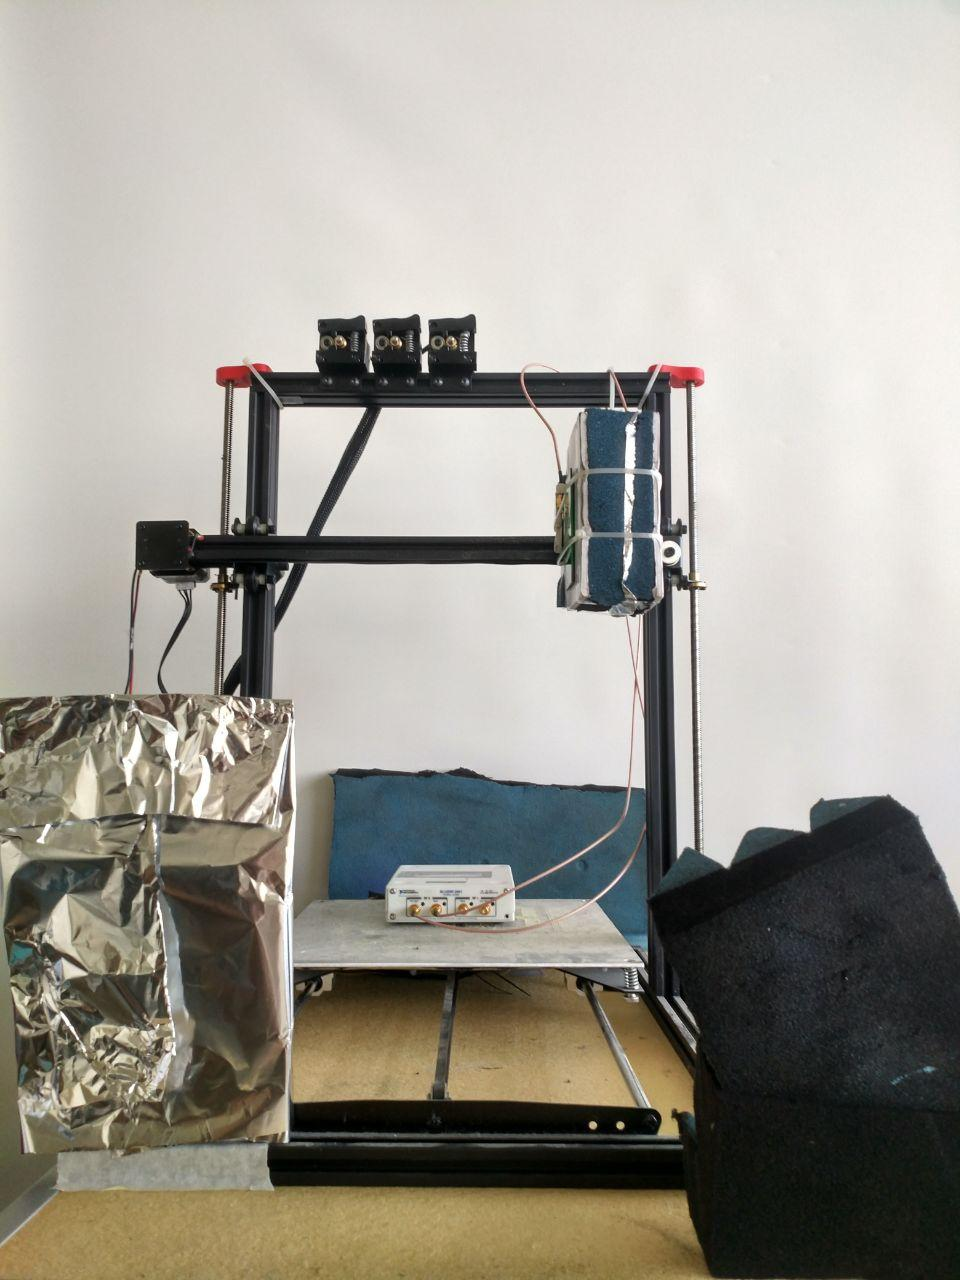
\includegraphics[scale=0.5]{figures/Rig2.jpg}
    \caption{RF Imaging Rig}
    \label{fig:RF_Imaging_rig}
\end{figure}


\chapter{Timeline \& Progress}
\section{Milestones}
\iffalse
\begin{itemize}
    \item Literature Survey
    \item Preparation Report Submission
    \item Progress Report Submission
    \item Final Report Submission
    \item Presentation
    \item Poster
    \item Toolkit Testing and Software Training
    \item gr-radar \acrshort{poc}
    \item Simulation Creation
    \item WiFi Image Creation
    \item RSSI Data Set Creation
    \item Analysis of Data Sets
    \item Basic Classification
    \item Create Hardware Setup for Presentation
    \item Final Submission
\end{itemize}
\fi
\begin{table}[H]
\centering
\caption{Milestones and Products}
\begin{tabular}{clccl}
\hline
\# & Name                                                                              & Deadline   & Hours  & Measurable Outcome                                                         \\ \hline
1  & Literature Survey \cmark                                                                 & 05/11/2019 & 100    & Knowledge                                                                  \\
2  & Prepartion Report \cmark                                                                 & 12/12/2019 & 48     & The Report itself                                                          \\
3  & \begin{tabular}[c]{@{}l@{}}Toolkit Testing and\\ Software Training\end{tabular}  \cmark & 12/12/2019 & 100    & Ability to Work                                                            \\
4  & GNU-Radio Gr-Radar \cmark                                                               & 27/12/2019 & 15     & \acrshort{poc}                                                                        \\
5  & Progress Report    \cmark                                                               & 24/01/2019 & 50     & The Report itself                                                          \\
& COVID-19 TIME & 03/2020 - 04/2020 & COVID-19 TIME &\\
6  & Simulation Creation \cmark                                                               & 05/2020 & 100    & Simulation                                                                 \\
7  & RSSI Data Set Creation \cmark                                                           & 05/2020    & 100    & Raw Data Set                                                               \\
8  & WiFi Image Creation    \cmark                                                           & 06/2020    & 200    & Images                                                                     \\
9  & \begin{tabular}[c]{@{}l@{}}Optional\\ Basic Classification\end{tabular}      \xmark     &     & Future Work    & \begin{tabular}[c]{@{}l@{}}Inferences of \\ Basic Environment\end{tabular} \\
10 & \begin{tabular}[c]{@{}l@{}}Optional\\ Analysis of Data Sets\end{tabular}  \xmark        &    & Future Work    & \begin{tabular}[c]{@{}l@{}}Inferences of \\ Environment\end{tabular}       \\
11 &  Reconstructed Images \cmark        &  08/2020 & 200    & Recognizable Object Image \\
12 & \begin{tabular}[c]{@{}l@{}}Create Hardware \\ Setup for Presentation\end{tabular} \cmark & 06/2020    & 50   & Hardware Setup                                                             \\
13 & Poster         \cmark                                                                   & 06/2020    & 60     & A Commercial Poster                                                        \\
14 & Presentation   \cmark                                                                   & 06/2020    & 60 & PPT and Videos                                                             \\
15 & Final Submission \cmark                                                                 & 08/2020    & 150 & Outstanding Project                                                        \\ \hline
\end{tabular}

\end{table}


\iffalse
\section{Measurable Products}
\begin{itemize}
    \item Formulating Methods and techniques
    \item Hardware Setup
    \item Simulation File
    \item Implementation Codes
    \item Experimentation Results
    \item Data Sets
    \item Data Sets Coding
    \item Classification of Environment
\end{itemize}
\fi
\pagebreak
\section{Risk Management}
\begin{itemize}
\item In retrorespect, a global pandemic such as the Novel Corona-virus 2019, a remote environment could be help.
    \item Some of the possible techniques are based on frequencies that we cannot generate (higher than 6GHz). We are going to use \gls{sdr}s that are limited by 6GHz. Hence, this is a risk.
    \newline  
    \newline In case of the embodiment of this risk, our solution is to fallback to a \gls{rssi} triangulation technique which is more implementable.
    \newline  
    \item The \gls{wifi} imaging algorithm requires a large antenna array in order to produce an image of the surrounding sensor environment. This can not be done with the equipment we have in hand. The article \cite{Scott:EECS-2017-191} also suggests a sparse antenna array implementation but with a trade-off in resolution.
    \newline
    Since we can only utilize up to $4\times 4$ \gls{mimo} with our \gls{sdr} by joining 2 devices as a single transmitter, this might be a risk. 
    We could end up with a low-resolution image with a small amount of information to relay on. \newline
    \newline
    The solution is to put more emphasis on information gained from other methods during the surrounding sensor environment inference (such as \gls{rssi} triangulation).

    \item Our project is very ambitious relative to our colleagues' final projects. Therefore, time is an influential resource, shortage of time will cause a partial implementation or lesser informative structure. 
    \newline
    \newline
    Hence, our solution is to first implement the simpler methods and algorithms in order to gain fundamental information to be used as a data-set.
    
    \item We are limited by time and space, that is, we can use a limited amount of environments (rooms) in our data-set gathering. This might not be enough to be useful to infer other environments.
    \newline
    \newline
    Our solution is to simulate the algorithms using \acrshort{rf} simulation software to train our model and gather more information using these simulations. 
\end{itemize}

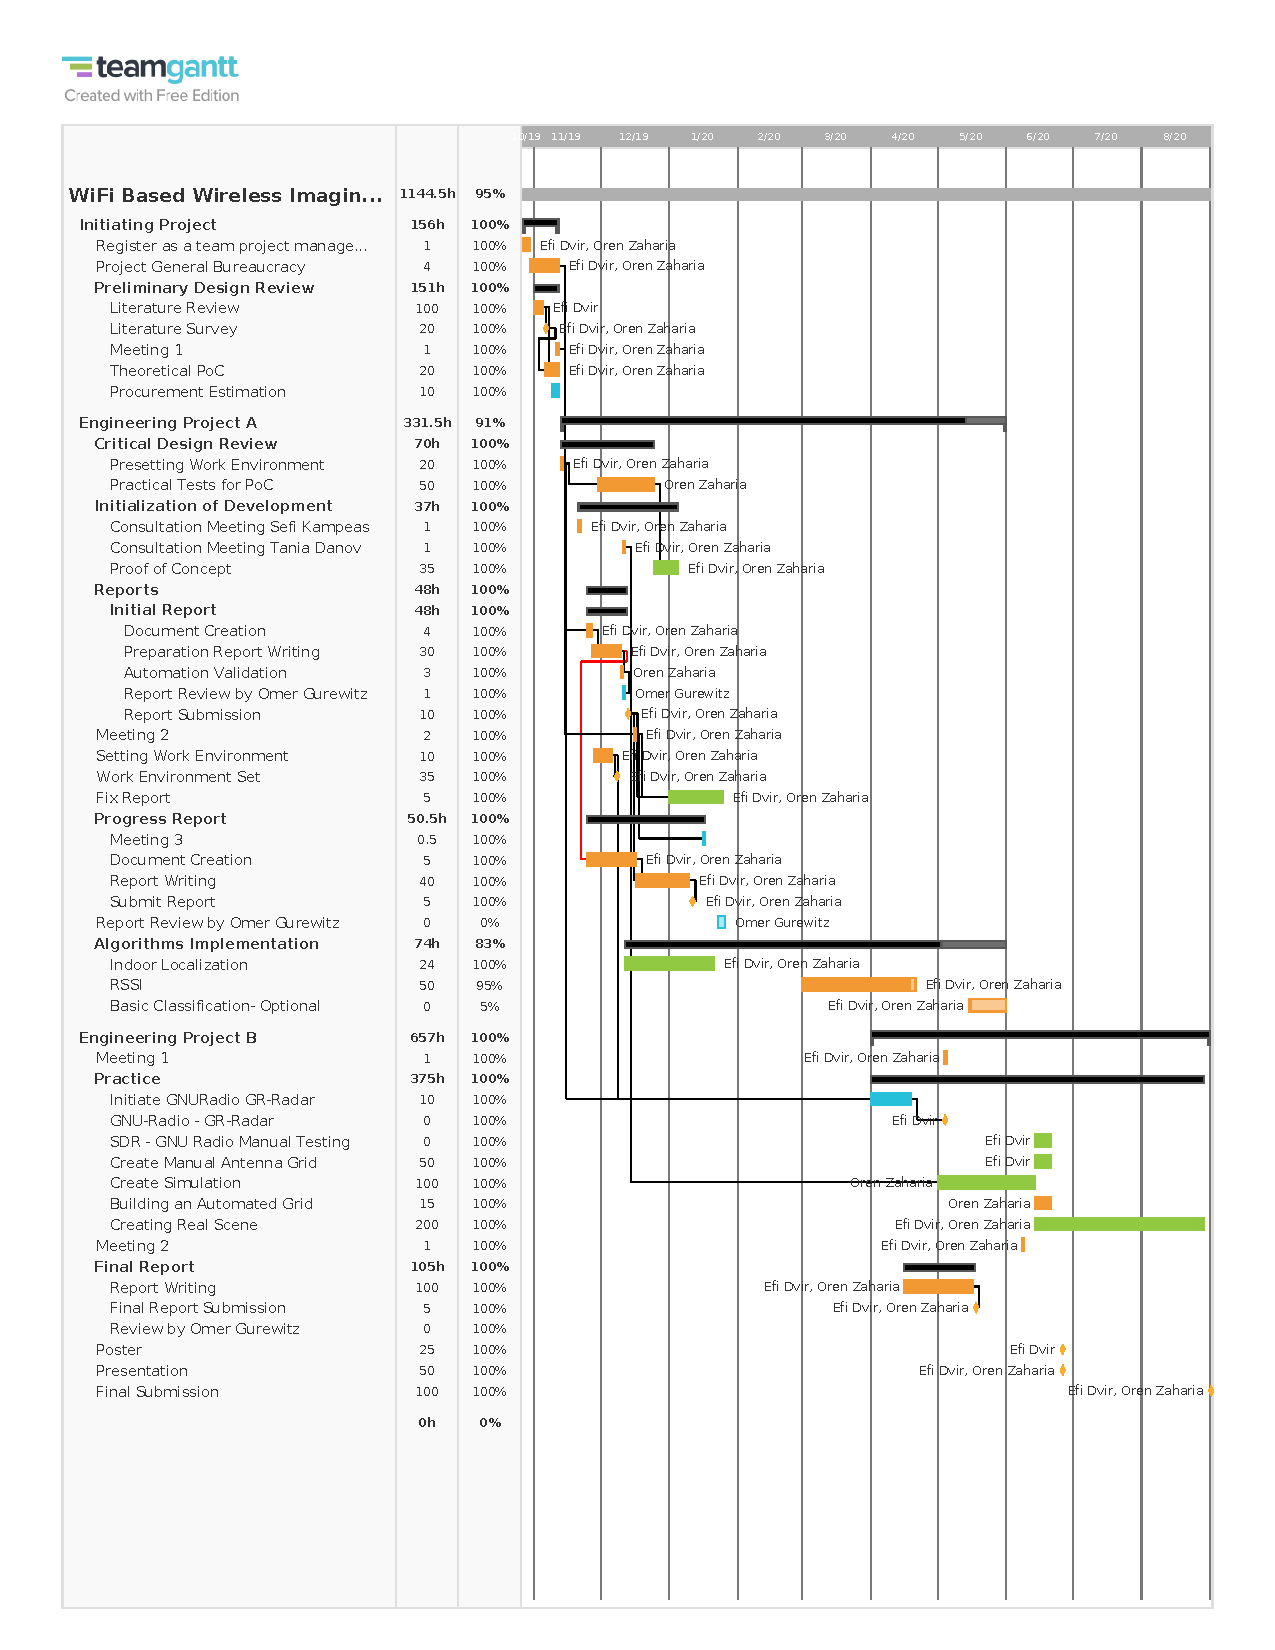
\includepdf[scale=0.68,pages=1,pagecommand=\section{Gantt}]{WiFi_Based_Wireless_Imaging_andPositioning_for_WSN.pdf}
%%%\chapter{Individual Contributions}%%%

%%%\chapter{Acknowledgements}%%%

%%%\chapter{Appendix}%%%

%%%\chapter*{Nomenclature}%%%

%%%\addcontentsline{toc}{chapter}{Nomenclature}%%%
\chapter{Testing \& Experimentation}

\section{RF Imaging experiments}
Before implementing the proposed methods we first had to prove their feasibility. Each concept involved in the method's functionality was first tested and proved to generate expected results. The following are the tests and experimentation made to show proof of concept.
\subsection{Phase vs. Distance}
In order to show that phase and distance are directly related, we constructed a basic transmitter-receiver flow chain in \gls{gnu}-Radio and along with an \gls{sdr} as hardware, the following experiment was made. 
\newline
The transmitting and the receiving antenna were placed about one meter apart and a sine wave signal was transmitter between them in a loop-back configuration. Slowly distancing them apart while simultaneously observing the transmitted ad received sine wave. 
Afterward, we introduced a mediator along the path in the form of a reflective aluminum surface. As showed in \ref{fig:phase_object}, the object in the path was slowly moved away from the antenna array elongating the radio path distance, this resulted in a visible subtle change in phase.
\begin{figure}[H]
\centering
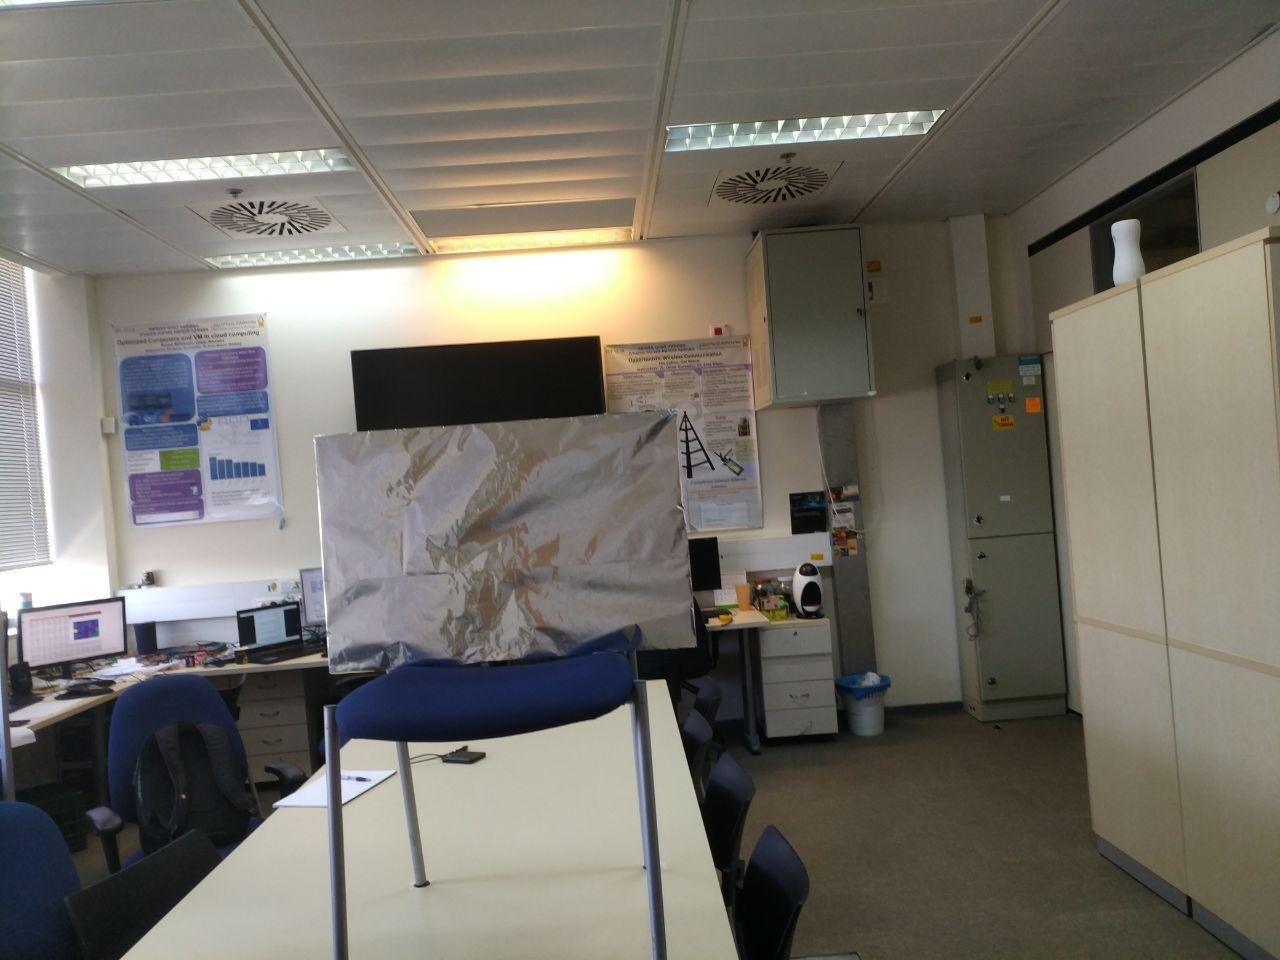
\includegraphics[width=5cm,keepaspectratio]{figures/phase_distance1.jpg}
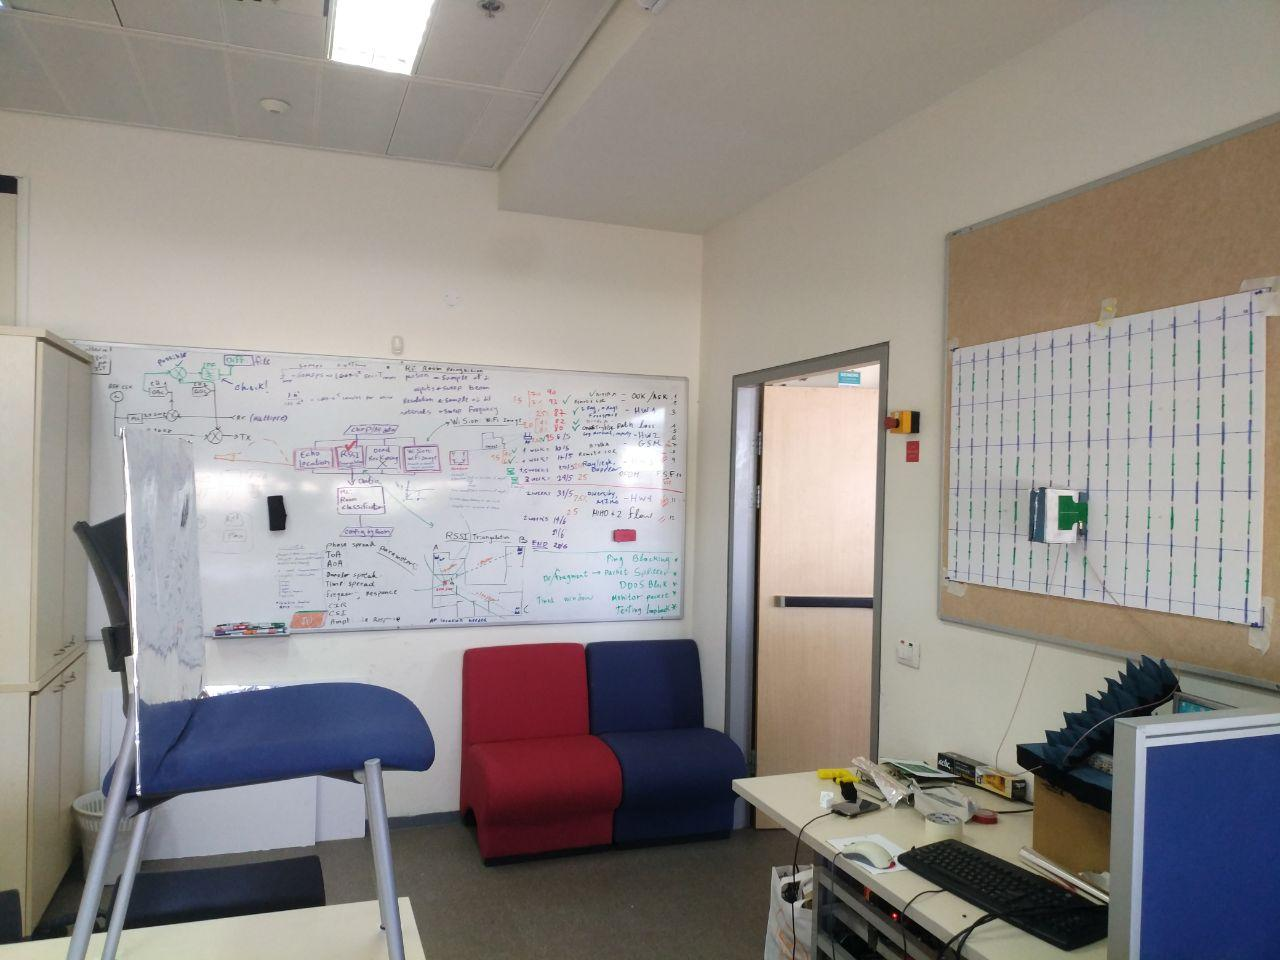
\includegraphics[width=5cm,keepaspectratio]{figures/phase_distance2.jpg}
\caption{Reflective object used for testing}
\label{fig:phase_object}
\end{figure}
\subsection{Distance vs. Power}
It is well known that radio signals traveling in space are effected by several factors and are attenuated by them. According to the free-space path loss propagation model, the distance the signal traverses is directly related to the amount of attenuation it experiences.  

\begin{equation}
    P_r=P_t\frac{G_tG_r\lambda^2}{(4\pi d)^2}
    \label{equ:fspl}
\end{equation}

In order to better understand the power that we need to transmit we conducted an experiment in order to guarantee that the received power is within the the dynamic range limits of the Rx input of the SDR.
We transmitter a signal withing a gain range between 0 and 70 and found that signals with a gain under 40 will be insufficient to traverse the entire room while a signal with again above 65 will distort the input and will cause inter-modulation. Therefore, a gain of 60 was decided as the base case of the entire implementation.
\newline
\newline


\subsection{Phase Comparator Vs. I\&Q}
In order to deduce the distance from objects, the implementation had a basic requirement - detect the phase difference between the transmitted signal and the received. Since our entire implementation is based on an \gls{sdr} we are limited to a mostly software implementation. Therefore, our first approach to phase detection was to using a phase comparator block as a part of the \gls{gnu}-Radio flow.
\newline
\newline
We found the gr-phase-comparator implementation of a phase comparator block in \gls{gnu}-Radio in 
\url{https://github.com/jettero/gr-phase-comparator} by Paul Miller aka jettero.
\begin{figure}[H]
    \centering
    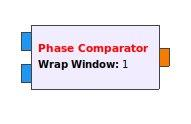
\includegraphics[scale=0.55]{figures/phase_comparator_block.jpg}
    \caption{gr-phase-comparator phase comparator \gls{gnu}-Radio block }
    \label{fig:phase_copmarator}
\end{figure}
This block compares the phase of two complex signal inputs and outputs the differential in phase as a float. This is done iteratively as a stream of values and the output can be wrapped in a time window to estimate the number of cycles. At a wrapped window of 1, the phase can be only in the range of $-\pi$ to $\pi$. This phase difference reading was to be combined with the relative amplitude received from the Rx input (the sampled reflected signal) to create the input to the \gls{rma} image reconstruction. 

\begin{figure}[H]
    \centering
    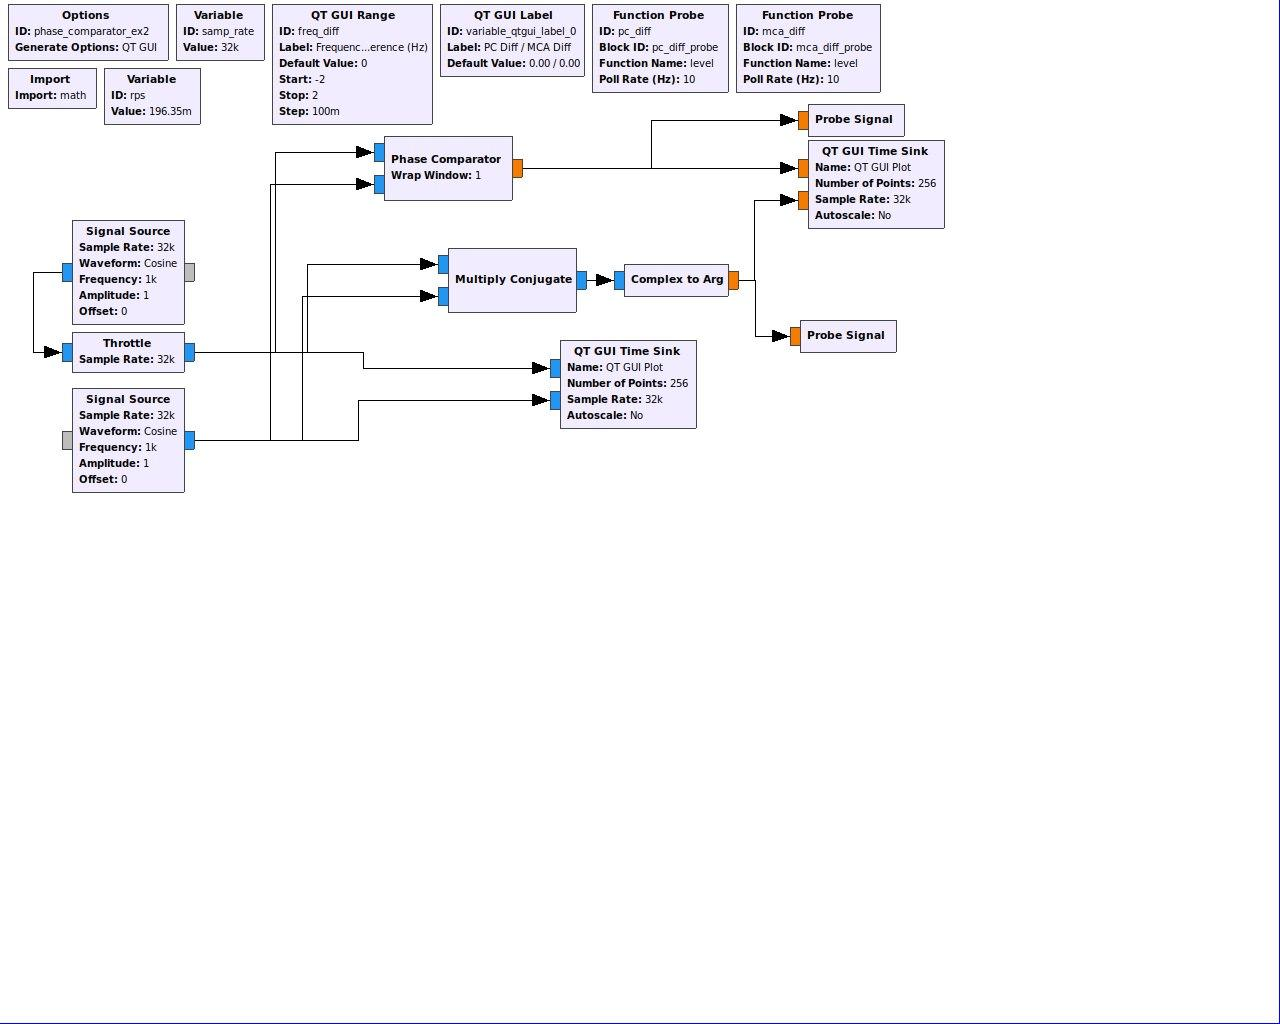
\includegraphics[trim=0 520 0 0,clip,scale=0.4]{figures/phase_comp__flow.jpg}
    \caption{RF chain flow - sampling reflections}
    \label{fig:phase_chain}
\end{figure}
Figure \ref{fig:phase_chain} showes the \gls{gnu}-Radio flow graph for sampling a single \acrshort{cw} base-band signal. This is for a single position in the \gls{rma} antenna array. 
Using this concept we went to implement the system using an \gls{sdr}, we made many tests in order to obtain the correct measurements needed for the \gls{rma} image reconstruction.
\begin{figure}[H]
    \centering
    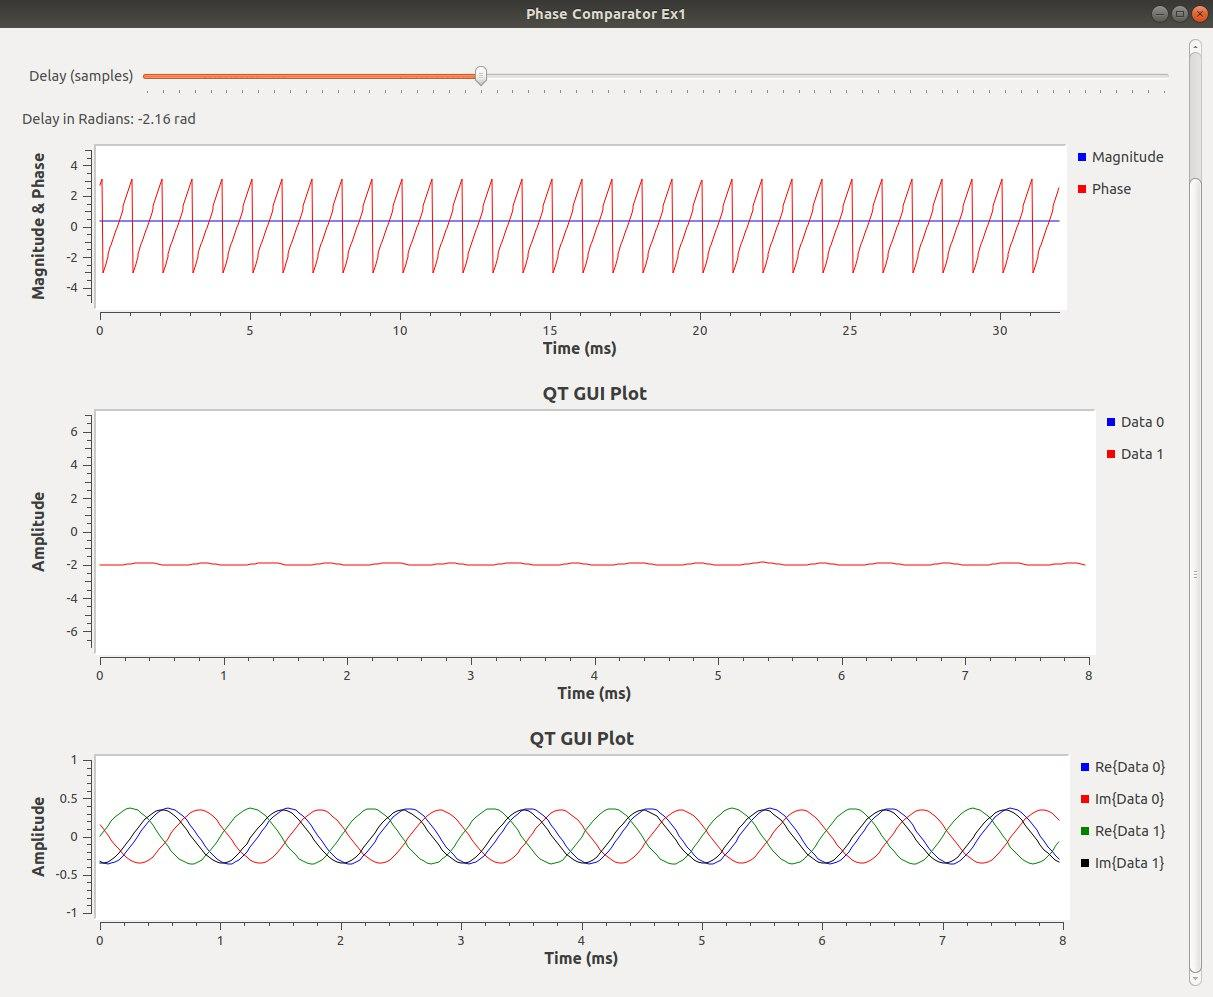
\includegraphics[scale=0.18]{figures/Phase_magnitude.jpg}
    \caption{Phase and Magnitude live \gls{sdr} mesurments}
    \label{fig:phase_magnitude}
\end{figure}
\begin{figure}[H]
    \centering
    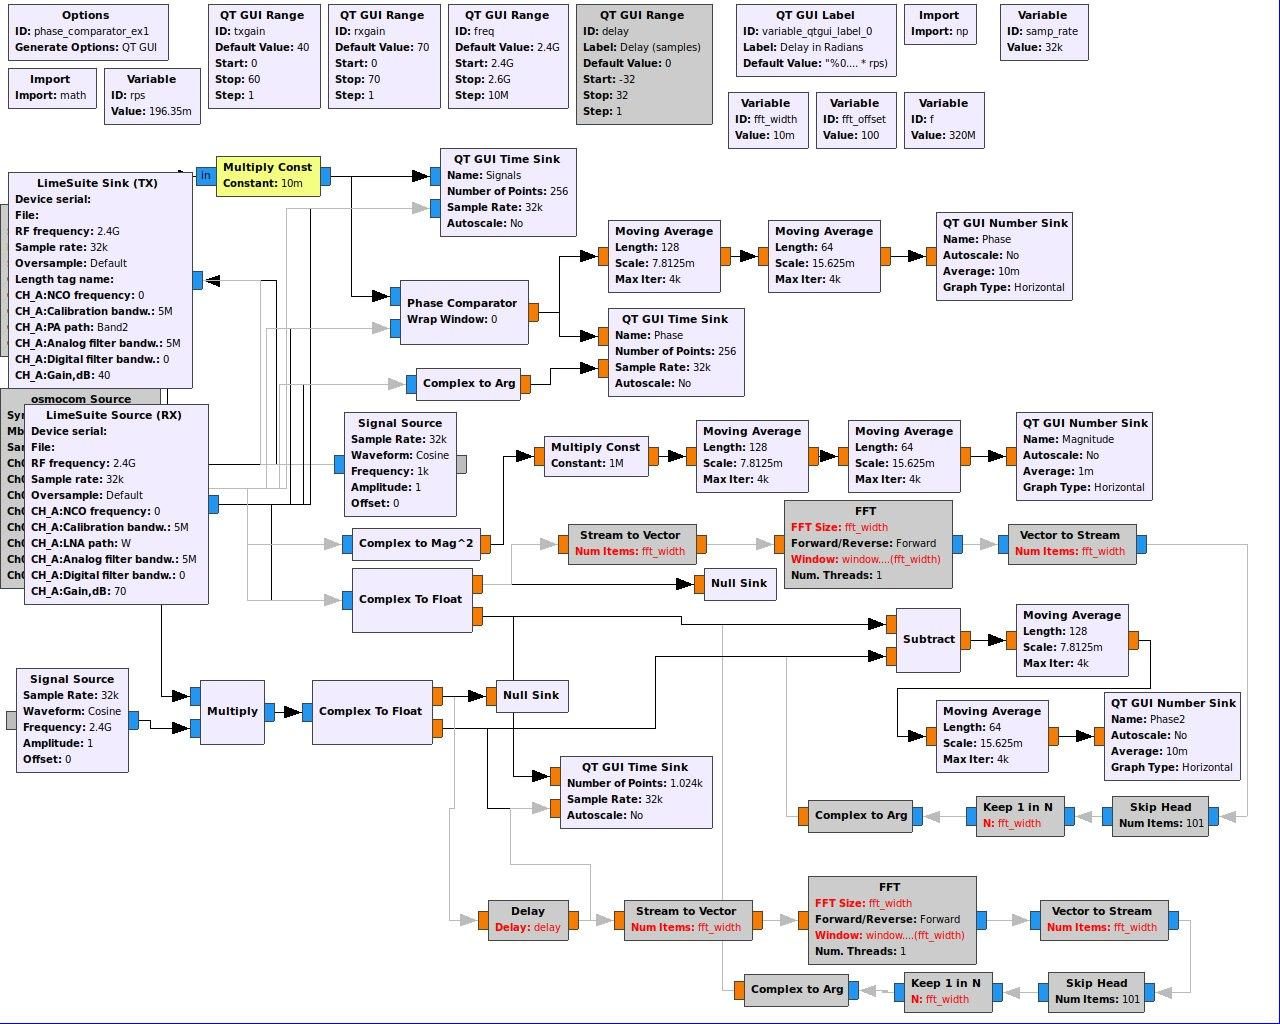
\includegraphics[trim=0 14 10 0,clip,scale=0.3]{figures/phase_comperator_testing.jpg}
    \caption{Tests preformed using the gr-phase-comparator}
    \label{fig:phase_tests}
\end{figure}
After testing the functionality of the gr-phase-comparator we came to an understanding that to implement the concept on an \gls{sdr} where most functionality is implemented in software, we could use a different approach.


\begin{figure}[H]
    \centering
    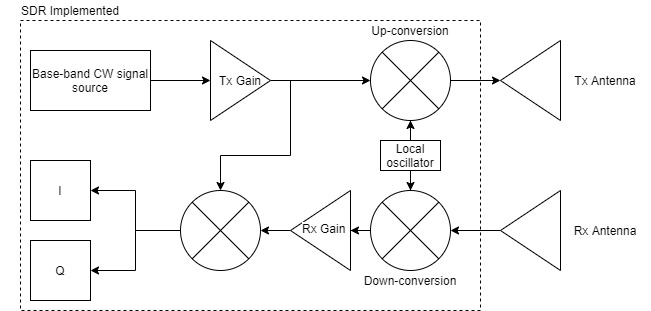
\includegraphics[scale=0.5]{figures/chain.jpg}
    \caption{RMA sampling \gls{rf} chain}
    \label{fig:rf_chain}
\end{figure}

Our implementation led us to an understanding that since the signal is upconverted and downconverted by the same oscillator withing the \gls{sdr}, the domain we are working in would only be in base-band. Since both Rx and Tx signals are conversion-synced we can multiply the signals (like using a mixer) and the result would generate a base-band signal. If there are no differences in time or frequency we would obtain a 0V \acrshort{dc} level. Where there are differences in time (and therefore in phase) we would obtain a very low-frequency shift from DC. Since our signals are already complex we could obtain the Phase and Magnitude (from the I \& Q components) as required by the \gls{rma} in order to reconstruct an image. 

\begin{figure}[H]
    \centering
    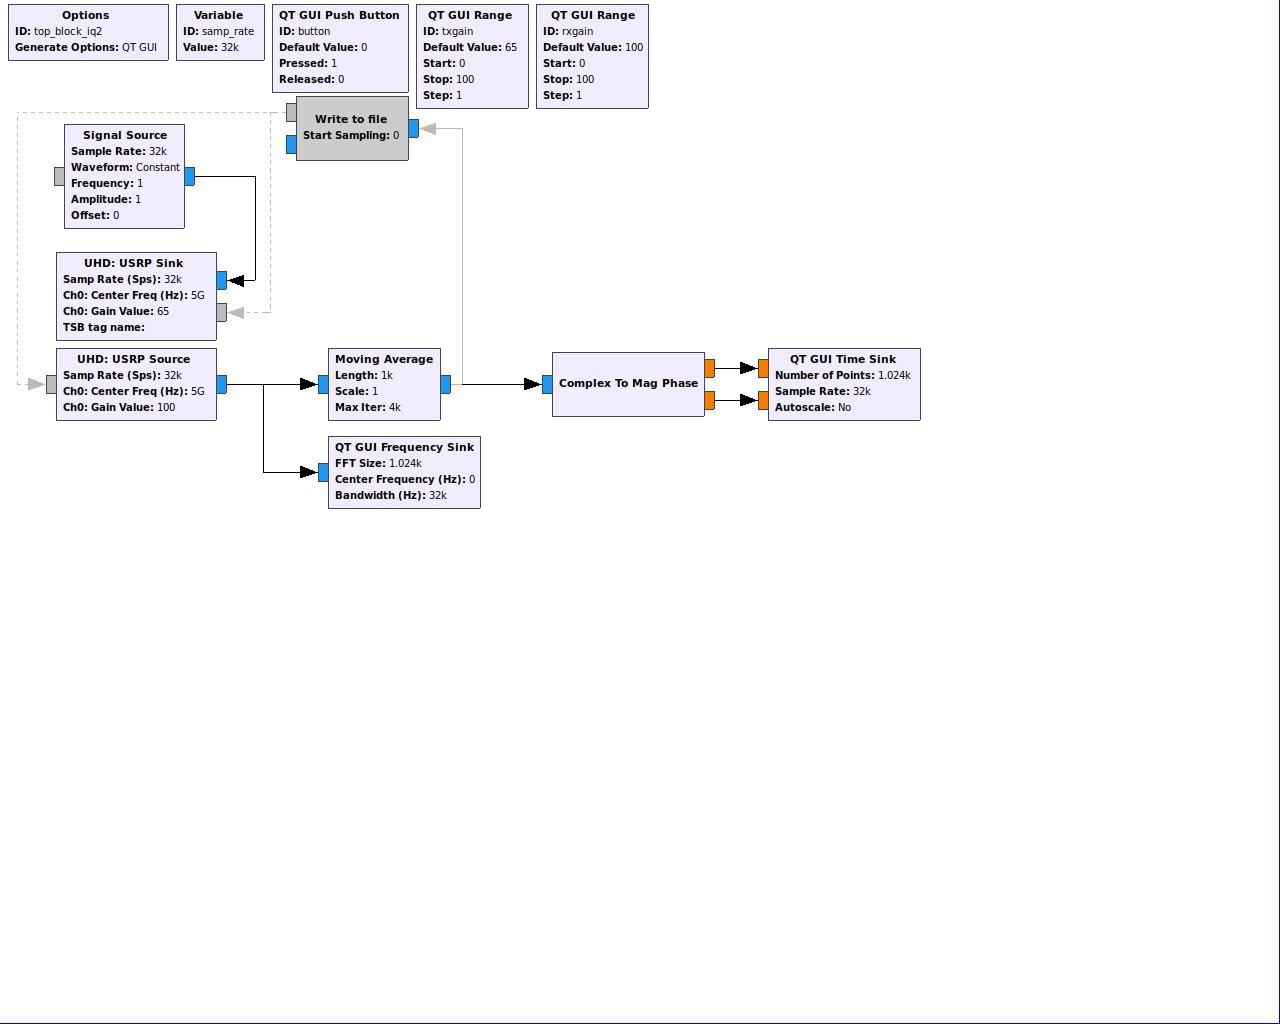
\includegraphics[trim=0 515 10 4,clip,scale=0.4]{figures/SImplified_phase_testing.jpg}
    \caption{Simplified semi-automatic I \& Q componetes mesurments}
    \label{fig:Simplified_testing}
\end{figure}

These Phase and Magnitude are simple float \acrshort{dc} values which allow this measurement design flow to be very undemanding in processing power and sample rate.

\subsection{The Effect of Disturbances}
During most experiments, we noticed the measurement setup is very susceptible to subtle changes in the room. That is, a slight movement of objects in the room has a significant effect on the measurements taken.
Therefore, we had to clear the room of any disturbances that could harm the results of our experiments. If a person would step into the room it could change the outcome of the image. 
\newline
\newline
To avoid disturbances we closed lab 511 in favor of our experiment and banned all from entering during active measurement. We also pointed our rig to an "open space" (Figure \ref{fig:open_space}) so it would be measuring the objects we intended and not objects around the room.
\begin{figure}[H]
    \centering
    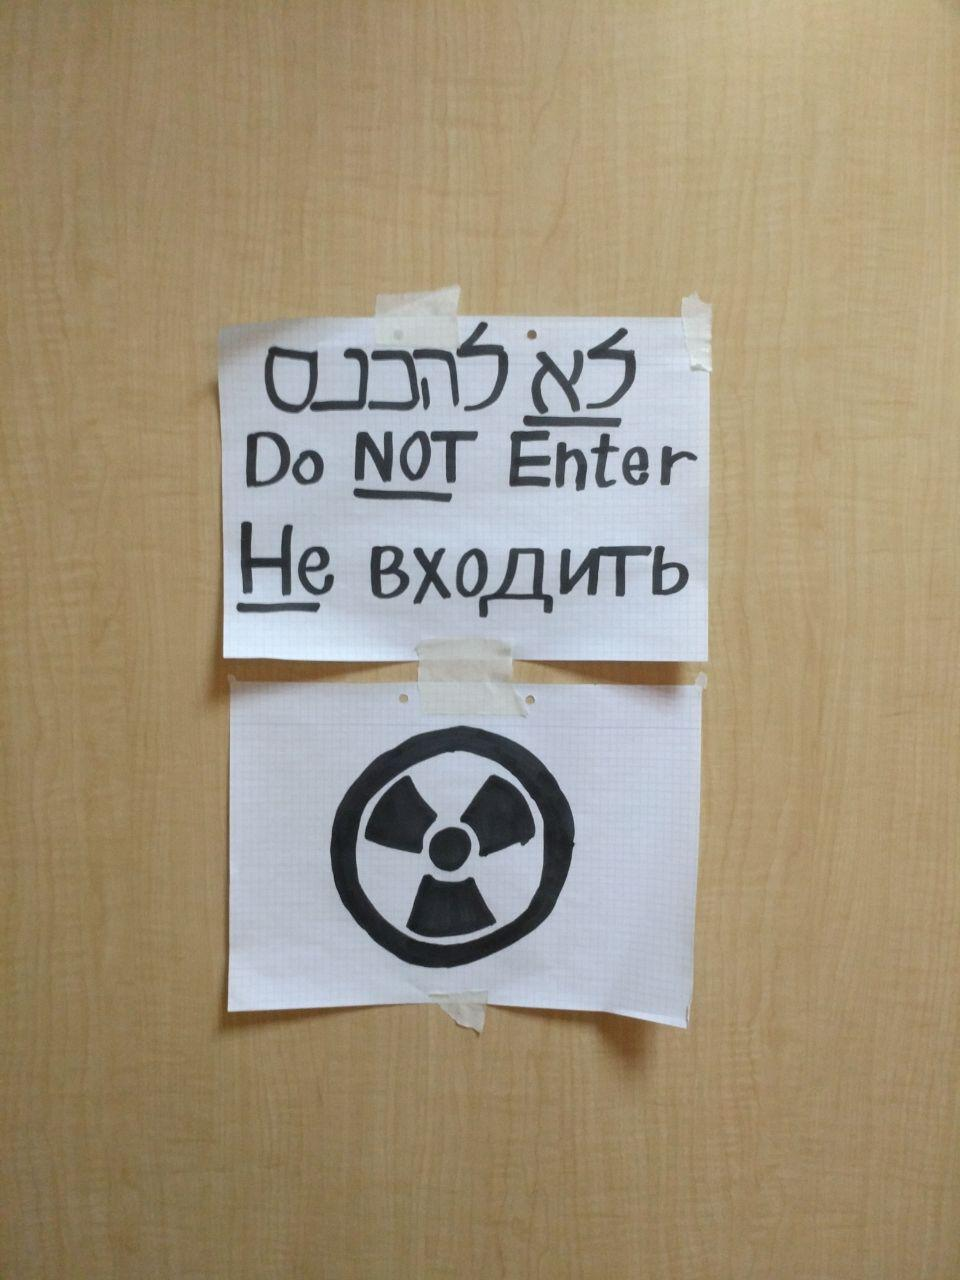
\includegraphics[trim=0 60 10 80,clip,scale=0.4]{figures/dont_enter.jpg}
    \caption{Lab 511 do not enter sign}
    \label{fig:dont}
\end{figure}
\begin{figure}[H]
    \centering
    \includegraphics[trim=0 60 10 80,clip,scale=0.4]{figures/pg}
    \caption{Lab 511 "Open Space"}
    \label{fig:open_space}
\end{figure}



\subsection{Motion} 
\label{motion}
Due to the effect of disturbances, we found that we could use the same setup for identifying if there is movement in the scanned room. A person walking and moving in the vicinity of the scanner would induce a significant change and instability in the phase and power of the receiving signal for a single point in the antenna array. Thus, it is fairly easy to identify movement using the same sensing technique we introduced. To identify movement periodic samples are taken in small time intervals. If the measured phase differs significantly, something is moving.

\subsection{\acrshort{cw} Vs. Frequency Modulated \acrshort{cw}}
Since radar signals are usually at high frequency, it is not possible to sample at Nyquist frequency since there are not analog to digital converter that can operate at such a high sample rate. In order to sample the signals, they are down-converted to base-band so to comply with Nyquist.
But with such a sample rate the time between each sample is grater that the time that a signal propagates through space. Thus, it is not possible to directly sample the signal's propagation time (from the transmission to reception).
\newline
\newline
In order to derive the propagation time, a simple trick can be used. By linearly increasing the frequency of the transmitted signal we can obtain the propagation time. The change in frequency correlates to the propagation time delay as seen in figure \ref{fig:fmcw}. This enables to measure the propagation time indirectly.
\begin{figure}[H]
    \centering
    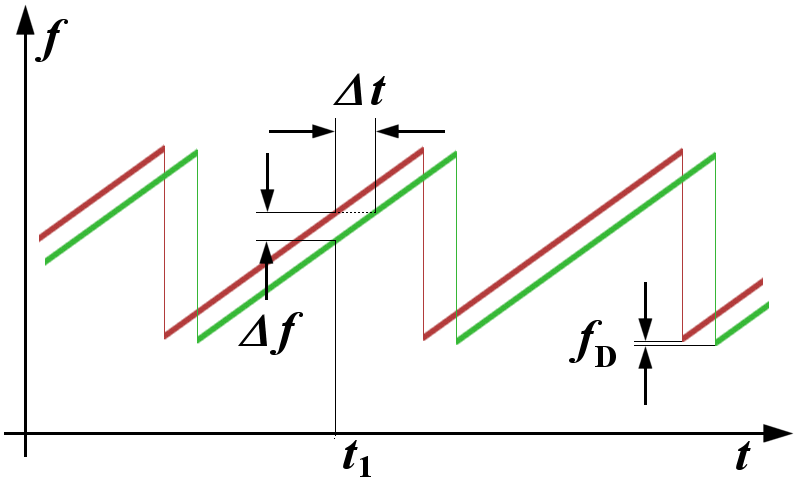
\includegraphics[scale=0.25]{figures/Fmcw_prinziple.png}
    \caption{FMCW Principal (transmitted in red received in green)}
    \label{fig:fmcw}
\end{figure}

We have made many tests with frequency-modulated \acrshort{cw} signals, seen in figure \ref{fig:FMCW}, yet we found that a stepped frequency change corresponds to the linear frequency change for the \gls{rma} and is simpler to calculate. Thus, we eventually chose the continuous-wave radar \cite{Continuous-wave_radar} approach as an input for the range migration algorithm.
In effect, the \gls{rma} uses different frequencies to distinguish different phase delays that correspond to the different propagation time of the transmitted signal.
\begin{figure}[H]
    \centering
    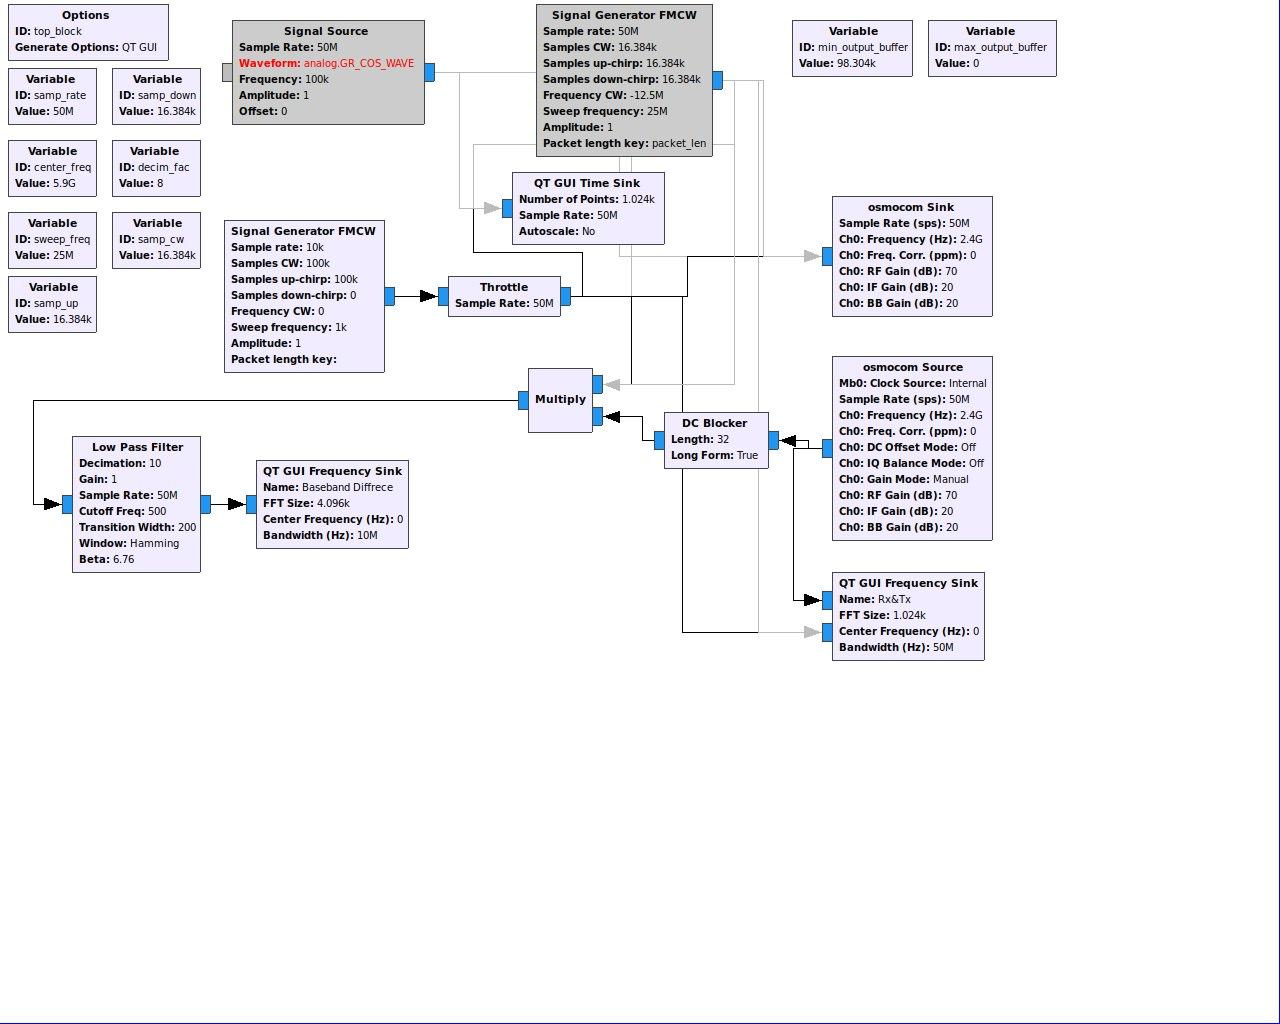
\includegraphics[trim=0 300 10 0,clip,scale=0.35]{figures/FMCW.jpg}
    \caption{FMCW scanning signal}
    \label{fig:FMCW}
\end{figure}
\subsection{Manual, semi-automatic and fully automatic measurements}
At the beginning of our \gls{rma} tests, in order to obtain measurements, we needed to change the position of the antenna array while changing the frequency in each position several times. 


\begin{figure}[H]
    \centering
    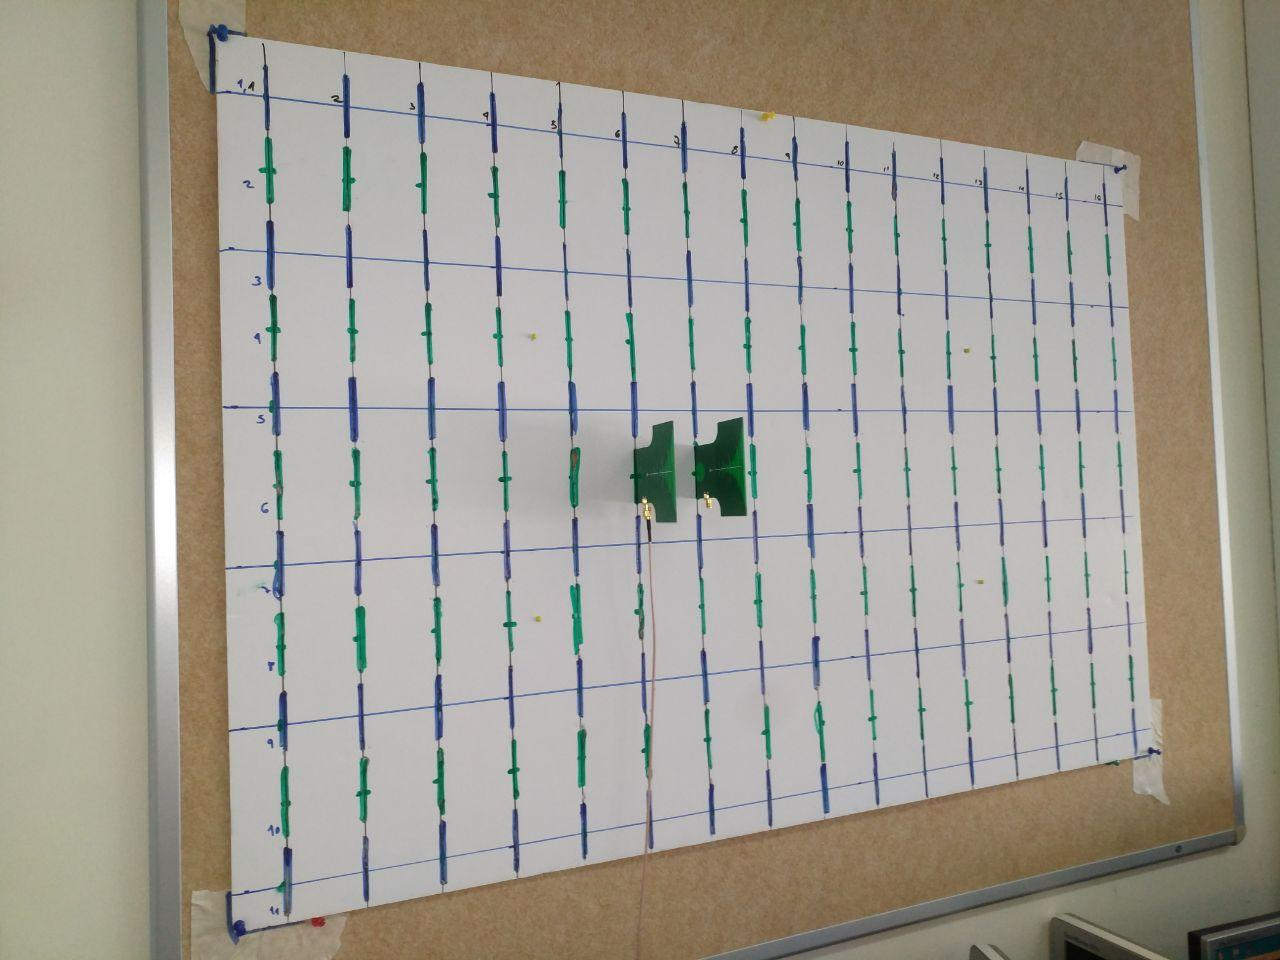
\includegraphics[scale=0.4]{figures/manual.jpg}
    \caption{Manual array positioning on a foam-board}
   
    \label{fig:foamboard}
\end{figure}


To do that we first started with manual measurements on a foam-board with 6.25cm slots spaces for the antennas to fit in (seen in figure \ref{fig:foamboard}). In each position (8X8) we would change the frequency manually from 4.95GHz to 5.6GHz and write down the I and Q values of the signal in an excel file. Once completed this file was used to feed the \gls{rma} image reconstruction code.

\begin{figure}[H]
    \centering
    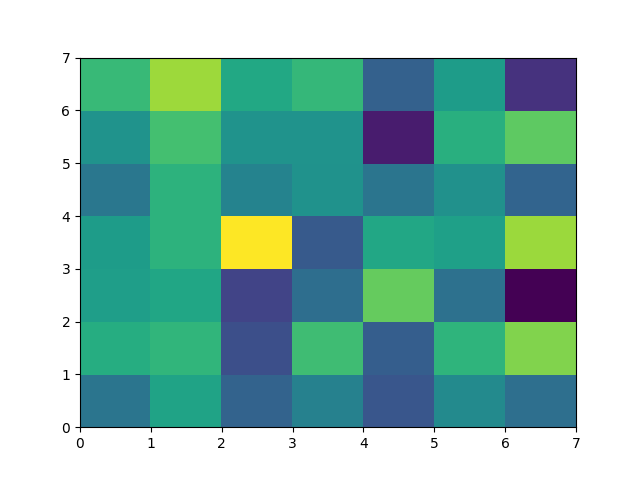
\includegraphics[scale=0.3]{figures/Figure_080620.png}
    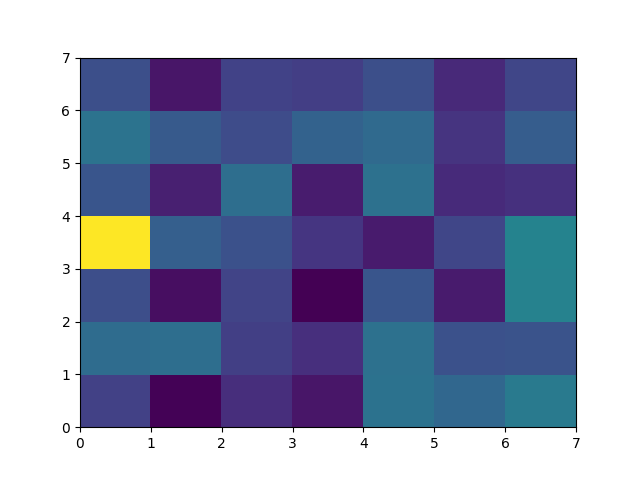
\includegraphics[scale=0.3]{figures/Figure_1_512.png}
    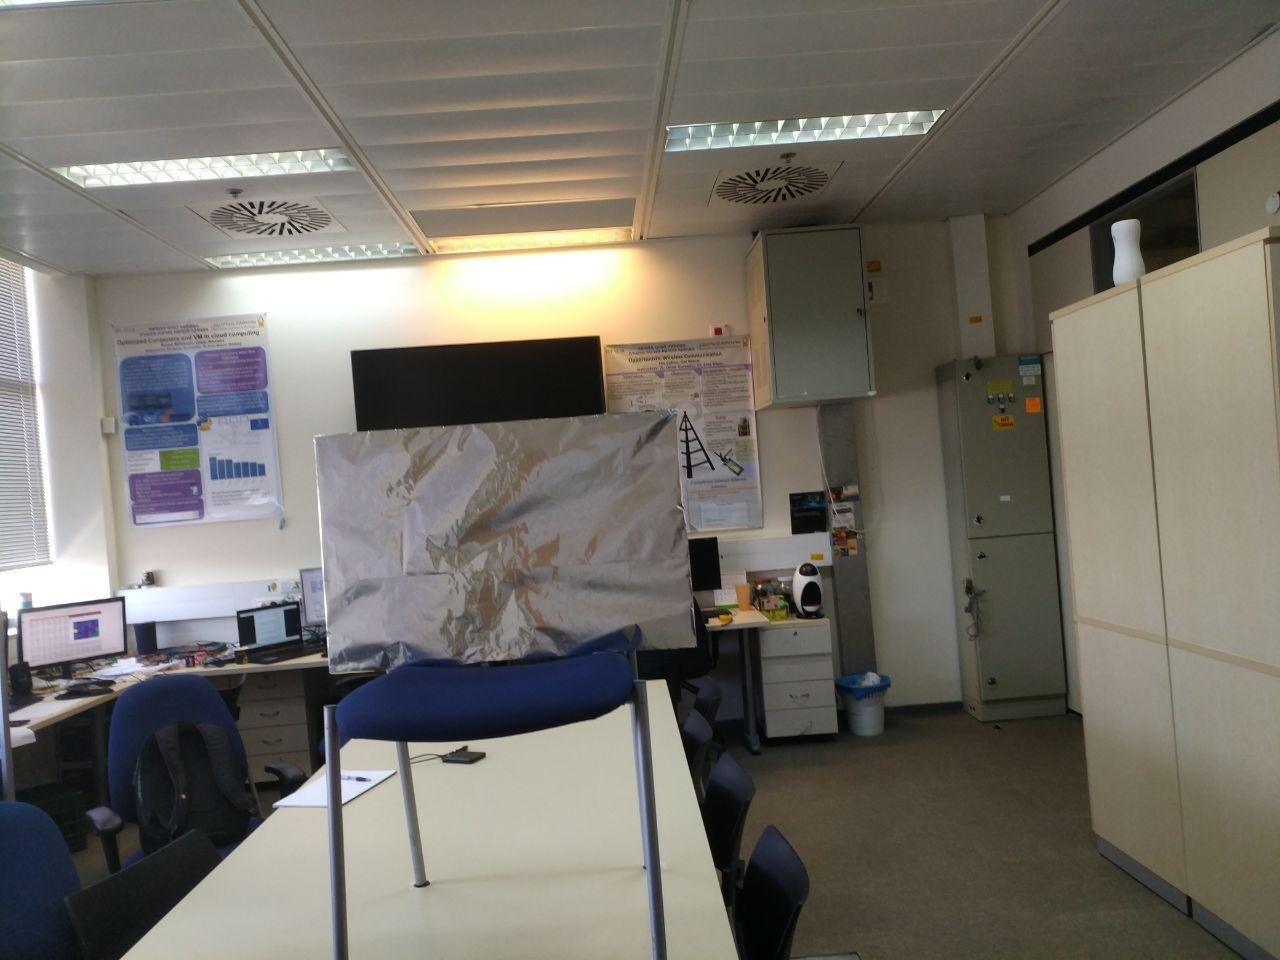
\includegraphics[width=4cm,keepaspectratio]{figures/phase_distance1.jpg}
    \caption{First \gls{rma} results}
    \label{fig:first_results}
\end{figure}

The first scans were of a rectangle aluminum reflector about 2m from the antenna array. The results in figure \ref{fig:first_results} were clearly insufficient to understand the dimensions and shape of the object yet the yellow pixel indicated that energy was indeed reflected form an object in front of the antenna array.
\newline
\newline
The manual scans were extremely laborious and took much time (about 5 hours for 64 positions and 16 frequencies). If we were to continue scanning we had to create a better scanning technique. So in the first stages of improvement, we created a semi-automated \gls{gnu}-Radio script to run the frequencies in each position and log the measurements directly to an excel file. 

\begin{figure}[H]
    \centering
    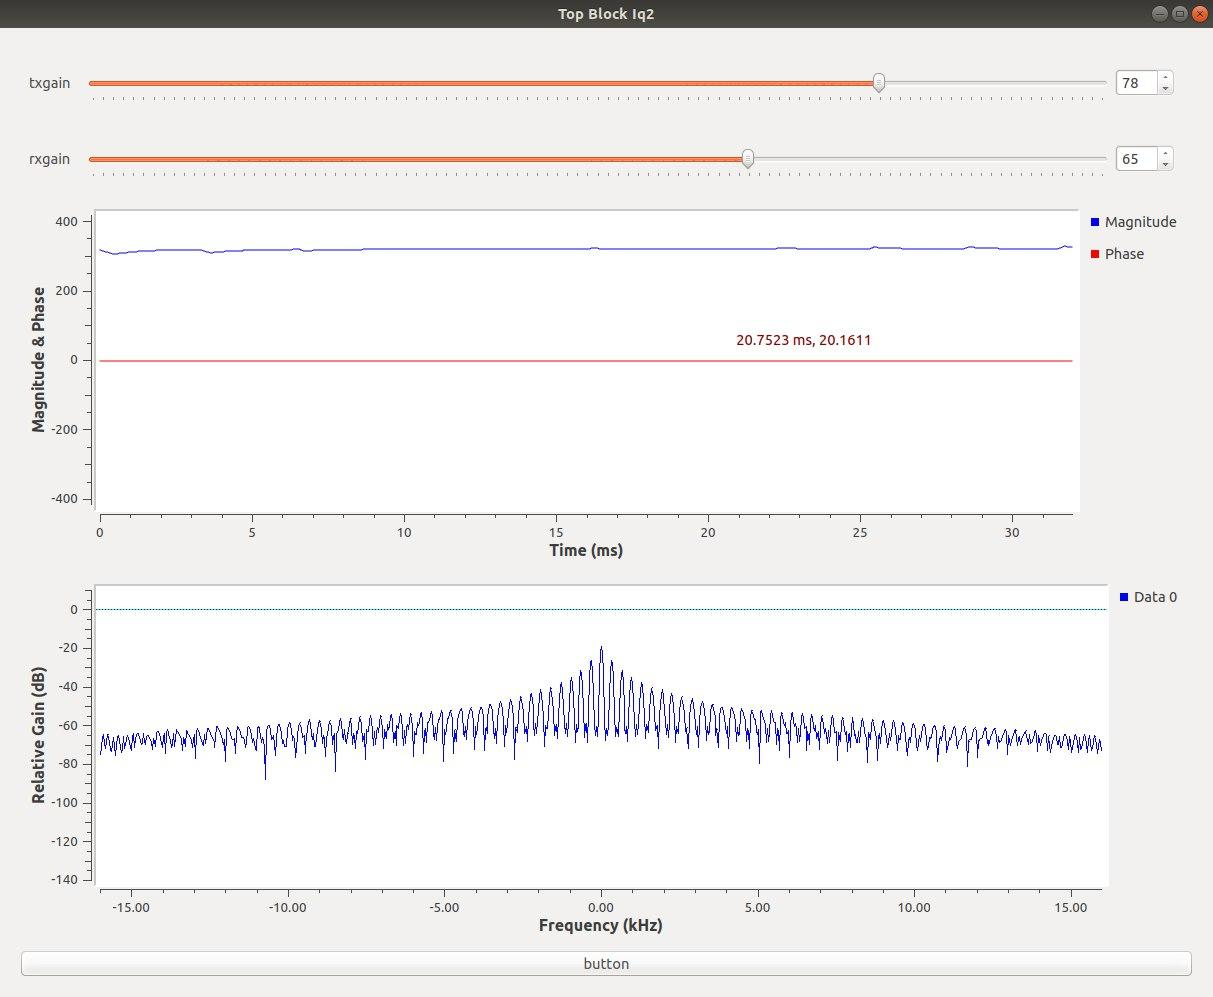
\includegraphics[scale=0.2]{figures/semi-auto.jpg}
    \caption{Semi-automatic \gls{gnu}-Radio scanning}
    \label{fig:semi-auto}
\end{figure}
 The script was written to a \gls{gnu}-Radio python block (seen in \ref{fig:Simplified_testing}) and with each 16 frequency changes the user had to press the GUI "Button" after chancing to the next position in the foam-board array.
 This the script was written to this block:
 
\begin{lstlisting}[language=Python,basicstyle=\scriptsize]

import numpy as np
import time
from threading import Timer
from gnuradio import gr
import pmt

flag = 0;
class blk(gr.sync_block):  # other base classes are basic_block, decim_block, interp_block
	"""Embedded Python Block example - a simple multiply const"""

	def __init__(self, start_sampling=1.0):  # only default arguments here
		"""arguments to this function show up as parameters in GRC"""
		gr.sync_block.__init__(
		    self,
		    name='Write to file',   # will show up in GRC
		    in_sig=[np.complex64],
		    out_sig=[np.complex64]
		)
		global flag
		self.freqs = [2.2e9,2.25e9,2.3e9,2.35e9,2.4e9,2.45e9,2.5e9,2.55e9,2.6e9,2.65e9,2.7e9,2.75e9,2.8e9,2.85e9,2.9e9,2.95e9]
		self.nfreqs = 16
		print('global flag', flag);
		if (flag == 0):
			self.cnt = 0

		self.boolTakeSample = False;
		self.boolTookSample = False;
		# if an attribute with the same name as a parameter is found,
		# a callback is registered (properties work, too).
		self.start_sampling = start_sampling
		self.message_port_register_out(pmt.intern('msg out'))
		def doTimer():
			if self.boolTakeSample == True:
				Timer(0.5, doTimer, ()).start();
				return;	
			if self.boolTookSample == False:
				self.boolTookSample = True;
				self.boolTakeSample = True;
				Timer(1, doTimer, ()).start();
				return;
			else:
				self.boolTookSample = False;
				self.boolTakeSample = False;			

			if self.cnt == self.nfreqs - 1:
				print("Press QT Button to Continute!");
				while (self.start_sampling == 0):
					continue
				self.cnt = -1;
				
			
			self.cnt += 1;
			print(self.cnt)
			d_ChgFreq = pmt.make_dict()
			d_ChgFreq = pmt.dict_add(d_ChgFreq, pmt.intern('freq'),pmt.from_double(self.freqs[self.cnt]) )
			self.message_port_pub(pmt.intern("msg out"), d_ChgFreq)
			Timer(2, doTimer, ()).start();
			return;

		if (flag == 0):
			Timer(1, doTimer, ()).start();
		flag = 1;

                
	def work(self, input_items, output_items):	

	        def get_result():
			if self.boolTakeSample == True:
				f = open(r'/home/lte/output2.csv', 'a+');
				f.write('{0},'.format(input_items[0][0]));
				print('{0},'.format(input_items[0][0]))
				f.close()
				self.boolTakeSample = False;
		get_result();
		output_items[0][:] = input_items[0];
		"""example: multiply with constant"""
		return len(output_items[0])
\end{lstlisting}

After several semi-automatic scanning, we came to the conclusion that the \gls{rma} image reconstruction is indeed working. Therefore we went a step further to fully automatize the scanning. We constructed the final imaging rig described in \ref{rig}, to which we had written new scripts that uses the \gls{usrp} native driver instead of the \gls{gnu}-Radio. We also had to write code to run the 3D printer movement between the acquirement of the measurements from the \gls{sdr}. This automation allowed us to increase the number of frequencies and positions resulting in a wider range of resolutions and detection abilities. Only after reaching this point the project that we were able to focus on the object recognition and the \gls{rma} itself.

\section{RSSI Triangulation}
Triangulation is a known procedure made by many devices in order to obtain a relative position in space. Before we were to pinpoint the location of out sensor we had to tweak and test several issues in the triangulation algorithm.
\subsection{Propagation Models}
The basis of triangulation is the knowledge of the distance to several anchor points in space. But in order to obtain the distance we had to apply a propagation model to the signal's path-loss. There are many propagation models \cite{Radio_propagation_model} to choose from, not all would result in good estimations to our indoor environment.
After constructing our setup (described in \ref{rssi_hardware}) we had to vary our propagation model to better fit the results obtained. Our environment was that of an office building making the free-space path-loss give us relative errors results.
The ITU model was found to be better for the testing environment in hand and was eventually combined with the simplified path-loss model.
The resulting indoor localization procedure is detailed in \ref{rssi_model}. 

\subsection{\gls{rssi}, \gls{ssid} and \gls{ap} capabilities}
All \gls{ap}s have different capabilities and we need to distinguish each \gls{ap} from another in order to apply the triangulation algorithm.
In order to obtain the information needed we had to turn to RFC5416 (\url{https://tools.ietf.org/html/rfc5416}).
For the Tx power of an \gls{ap} we found the Tx Power beacon frame in section 6.18 (\url{https://tools.ietf.org/html/rfc5416#section-6.18}):

\begin{verbatim}
6.18.  IEEE 802.11 Tx Power

   The IEEE 802.11 Tx Power message element value is bi-directional.
   When sent by the WTP, it contains the current power level of the
   radio in question.  When sent by the AC, it contains the power level
   to which the WTP MUST adhere.

        0                   1                   2                   3
        0 1 2 3 4 5 6 7 8 9 0 1 2 3 4 5 6 7 8 9 0 1 2 3 4 5 6 7 8 9 0 1
       +-+-+-+-+-+-+-+-+-+-+-+-+-+-+-+-+-+-+-+-+-+-+-+-+-+-+-+-+-+-+-+-+
       |    Radio ID   |    Reserved   |        Current Tx Power       |
       +-+-+-+-+-+-+-+-+-+-+-+-+-+-+-+-+-+-+-+-+-+-+-+-+-+-+-+-+-+-+-+-+
\end{verbatim}

This frame allows us to the Tx power and along with the \gls{rssi} calculate the path-loss for the specific Radio-ID (or \gls{ssid}.
\newline
\newline
For the \gls{rssi} information at the sensor (receiver), we found to be included in each IEEE 802.11 frame and thus could be extracted.  

\begin{verbatim}
     IEEE 802.11 Frame Info:  When an IEEE 802.11 frame is received from a
      station over the air, it is encapsulated and this field is used to
      include radio and PHY-specific information associated with the
      frame.

      The IEEE 802.11 Frame Info field has the following format:

      0                   1                   2                   3
      0 1 2 3 4 5 6 7 8 9 0 1 2 3 4 5 6 7 8 9 0 1 2 3 4 5 6 7 8 9 0 1
     +-+-+-+-+-+-+-+-+-+-+-+-+-+-+-+-+-+-+-+-+-+-+-+-+-+-+-+-+-+-+-+-+
     |     RSSI      |     SNR       |           Data Rate           |
     +-+-+-+-+-+-+-+-+-+-+-+-+-+-+-+-+-+-+-+-+-+-+-+-+-+-+-+-+-+-+-+-+

      RSSI:   Received Signal Strength Indication (RSSI) is a signed,
         8-bit value.  It is the received signal strength indication, in
         dBm.
\end{verbatim}

Once all the information needed to apply a triangulation algorithm was found to be in had we could start our implementation.

\chapter{Implementations}
\section{Achieved Objectives}
\subsection{\gls{rssi} Distance Measurements}
\label{rssi_model}
We've used two different formulas to estimate the distance of the \gls{wifi} client from its neighbors \acrshort{ap}. The first formula is given by the \acrshort{itu} \cite{wiki:itu_model}
\begin{equation}
    L=20\log_{10}f+N\log_{10}d+P_{f}\left(n\right)-28    
\end{equation}
where,\newline
$L$ the total path loss in dB.\newline
$f$ is the frequency in usage.\newline
$d$ the distance in meters.\newline
$n$ the number of floors between the two nodes.\newline
$P_{f}$ the floor loss penetration factor.\newline
$28$ a constant that is given in the model.\newline
\newline
Our interpretation to this model is given by 
\begin{equation}
    d=\exp\left(\log10\cdot\frac{L-20\log_{10}f-P_{f}\left(n\right)+28}{N}\right)
\end{equation}
where the results of the distance $d$ are shown in figure \ref{fig:esp_rssi}.
Another model by A.Goldsmith \cite[p.46]{goldsmith_2005}, simplified path-loss given by,
\begin{equation}
    P_{r}=P_{t}+K-10\gamma\log_{10}\left[\frac{d}{d_{0}}\right]
\end{equation}
where,\newline
$P_{r}$ is the received power (\gls{rssi}).\newline
$P_{t}$ is the transmitted power.\newline
$K$ is a unit-less constant that depends on the antenna characteristics.\newline
$\gamma$ is the path-loss exponent.\newline
$d_{0}$ is the refrenced distance [10-100]m.\newline

Our interpretation to this model is given by 
\begin{equation}
    d=\exp\left(\log10\cdot\frac{P_{t}-P_{r}+K}{10\gamma}\right)\cdot d_{0}
    \label{distance_simplified_equation}
\end{equation}

This implementation was done using the device branded by WeMos D1 and is given in figure \ref{fig:wemosd1}.
\begin{figure}[H]
\centering
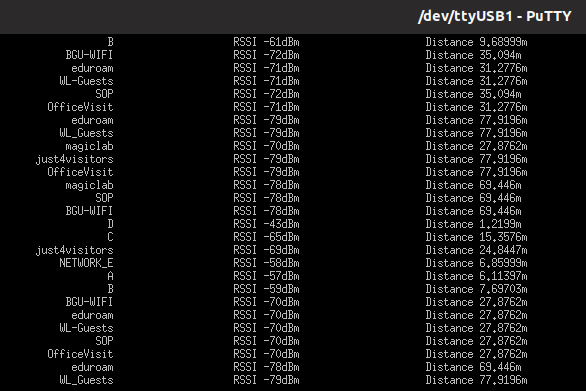
\includegraphics[width=12cm,keepaspectratio]{figures/esp_rssi.png}
\caption{Results of \gls{rssi} based distances}
\label{fig:esp_rssi}
\end{figure}
In figure \ref{fig:esp_rssi} appears a list of all the surrounding \acrshort{ssid}s broadcasted from nearby \gls{ap}s in range.
The list includes the \acrshort{ssid}, the \gls{rssi} and the calculated distance (using formula \
\ref{distance_simplified_equation}) respectively. 
The WeMos D1 node is running an operation system known as \href{https://micropython.org}{MicroPython}, and the python code that runs it, is at appendix \ref{apdx:wemos_python}.
\begin{figure}[H]
\centering
\includegraphics[width=8cm,height=6cm,keepaspectratio]{figures/wemos_d1.jpg}
\caption{\href{https://wiki.wemos.cc/products:d1:d1_mini}{WeMos D1 mini}}
\label{fig:wemosd1}
\end{figure}

\subsection{\gls{rssi} Indoor Localization}
This method described in \cite{Fundamentals_of_Wireless_Sensor_Networks} and is based on the previous paragraph, where the localization is calculated by the following equation
\begin{equation}
    \mathbf{A}\mathbf{x}=b
\end{equation}
where,\newline
$\mathbf{x}$ is the vector unknown sensor location  $\left(x,y\right)$ compared to the other anchors.
$\mathbf{A}$ is the matrix of the $n-1$ anchors compared to the sensor location, given by
\begin{equation}
    A=\left[\begin{array}{cc}
2\left(x_{n}-x_{1}\right) & 2\left(y_{n}-y_{1}\right)\\
2\left(x_{n}-x_{2}\right) & 2\left(y_{n}-y_{2}\right)\\
\vdots & \vdots\\
2\left(x_{n}-x_{n-1}\right) & 2\left(y_{n}-y_{n-1}\right)
\end{array}\right]
\end{equation}
$b$ is the vector of distances and locations of the other anchors and to the other anchors, given by
\begin{equation}
    b=\left[\begin{array}{c}
r_{1}^{2}-r_{n}^{2}-x_{1}^{2}-y_{1}^{2}+x_{n}^{2}+y_{n}^{2}\\
r_{2}^{2}-r_{n}^{2}-x_{2}^{2}-y_{2}^{2}+x_{n}^{2}+y_{n}^{2}\\
\vdots\\
r_{n-1}^{2}-r_{n}^{2}-x_{n-1}^{2}-y_{n-1}^{2}+x_{n}^{2}+y_{n}^{2}
\end{array}\right]
\end{equation}

\begin{figure}[H]
    \centering
    \includegraphics[height=5cm,height=5cm,keepaspectratio]{figures/Room512.pdf}
    \caption{\gls{rssi} triangulation inside 512/37 lab}
    \label{fig:rssi_triag_512}
\end{figure}
Given the figure \ref{fig:rssi_triag_512} of our space, the indoor localization, is calculated using the interpreted equation
\begin{equation}
    \left(x,y\right)=\left(\mathbf{A}^{T}\mathbf{A}\right)^{-1}\mathbf{A}^{T}b
\end{equation}
where, the distances $r_{i}$ are calculated using one of the model mentioned before, and the inverse of the matrices is calculates using the Moore-Penrose inverse methods that is pseudoinverse \cite{wiki:moorepenrose}.
The Jupyter notebook code is in the appendix \ref{apdx:jupyter_indoor}.
\newline
\newline
We placed 4 \gls{wifi} routers in lab 512 and 521 and measured their location using a measuring meter.  Each router broadcasts a \gls{ssid} (A, B, C, D) which serves as an anchor point in space. The algorithm is dependent on these points to calculate the estimated location of a sensor relative to these points.
\newline
\newline
Results showed an accuracy of about 0.3m.
\subsection{Radio Frequency Imaging}
The following is a description from Simon Scott's work \cite{Scott:EECS-2017-191} on Radio Frequency Imaging.
\subsubsection{Range Migration Algorithm}
Radio Frequency Imaging is the technology for capturing 3D images of objects and people in an indoor environment. Compared to many other imaging technologies, radio frequency imaging suffers from significantly lower resolution and the resolution is limited to half the wavelength of the carrier frequency. Therefore, microwave imaging is best suited to large indoor environments where only moderate resolution is required.

From sub-section \ref{Techniques Survey}, only one radio frequency imaging technique was found to be implementable in the time scope of this project and with the confinement of using a fairly standard WiFi-based radio.
Therefore, we have selected to focus on the work of Simon Scott \cite{Scott:EECS-2017-191} whose work relays on an algorithm for microwave imaging called range migration algorithm (\gls{rma}) which has its origin in seismic ground scanning. The range migration algorithm has its origins in acoustic imaging. It was first used in
geological surveying applications \cite{RMA_ground}, where acoustic waves are used to image underground
objects. It was also used in its early days for ultrasound medical imaging \cite{10.1007/978-1-4615-8210-6_18}. \gls{rma} takes into account the wavefront curvature, and can also be computed efficiently. This efficiency comes from the fact that the \gls{rma} uses the Dix approximation, i.e. only direct reflections are considered and multipathing is ignored. This approximation allows the algorithm to be expressed using Fourier transforms and computed using fast Fourier transforms (FFTs). \gls{rma} is also known as the backward-wave reconstruction algorithm \cite{10.1007/978-1-4615-8210-6_18}, as it forms an image by coherently integrating the reflected
wave over a synthesized aperture, and then back-projecting it into the scene. The \gls{rma} is
derived here from first principles for multiple different antenna array configurations.
The conventional 3-D \gls{rma} assumes a planar rectangular antenna array of colocated
transmit and receive antennas, with antennas spaced less than a wavelength apart. This
arrangement is the easiest to analyze and generally produces the highest resolution images.
\subsubsection{Variables and Coordinate System}
Figure \ref{fig:scene} establishes a unified coordinate system to aid in the explanation and derivation
of the different RMA variants. This coordinate system, as well as the common variables, are
defined as follows:
\begin{itemize}
    \item The antenna array lies in the xy-plane at $z = Z_0$.
    \item The transmitter transmits a continuous wave (\acrshort{cw}) at frequency $\omega$ (rad/s), that is discretely stepped from $\omega_{min}$ to $\omega_{max}$.
    \item $f(x, y, z)$ is the reflectively function of the scene, i.e. the image we are trying to recreate. Note that “imaging the scene” actually means finding the function $f$ that defines how well each point in the scene reflects microwaves.
    \item  $s(x_a, y_a, \omega)$ is the complex reflection recorded at antenna position $(x_a, y_a, Z_0)$ and at frequency $\omega$, when both the transmitting and receiving antennas are co-located.
    \item $k = \frac{\omega}{c}$ is the wavenumber of the transmitted signal.
    \item $k_x, k_y, k_z$ are the spatial frequency variables of $x, y, z$.
\end{itemize}
\begin{figure}[H]
    \centering
    \includegraphics[trim = 0 150 0 0, clip, scale=0.47]{figures/Scene.jpg}
    \caption{Scene geometry for the derivation of the range migration algorithm}
    \label{fig:scene}
\end{figure}
\paragraph{Co-located Range Migration Algorithm} Only two antennas in the array are active in the co-located algorithm at any one time: the transmitting antenna and its neighboring receive antenna. A continuous-wave (CW) signal is transmitted by the transmitter, which reflects off objects in the scene and this reflection is coherently recorded by the neighboring receiver. This is repeated for each frequency step from $\omega_{min}$ to $\omega_{max}$. After recording reflections $s(x_a, y_a, \omega)$ at all frequencies, the next two antennas in the array operate as the transmit/receive pair and the process is repeated.
The co-located algorithm assumes that the transmitting and receiving antennas are co-located (i.e. in the exact same position), but in practice co-location is approximated by having neighboring antennas act as a transmit/receive pair. Therefore, a common technique is to take position $(x_a, y_a)$ as the position halfway between the neighboring antennas.

\subsubsection{ Derivation of the colocated range migration algorithm}

The round-trip phase delay from transmit/receive antenna at $(x_a, y_a, Z_0)$ to point reflector in the scene at co-ordinate $(x, y, z)$ is:
\begin{equation}
    2k\times d, \text{where distance } d=\sqrt{(x-x_a)^2+(y-y_a)^2+(z-Z_0)^2}
\end{equation}
Attenuation effects due to path loss are ignored in the co-located range migration algorithm, as they are difficult to handle and have little effect on the resulting image quality \cite{weapon_detection}.
Therefore, if the point reflector at co-ordinate $(x, y, z)$ has reflectively $f(x, y, z)$, the response $s$ recorded at the antenna at frequency $\omega$ will be:
\begin{equation}
\label{eq1}
    s(x_a, y_a, \omega)=f(x,y,z)e^{-j2k\sqrt{(x-x_a)^2+(y-y_a)^2+(z-Z_0)^2}}
\end{equation}
By regarding the scene as a collection of point reflectors, the combined reflection recorded
at antenna $(x_a, y_a, Z_0)$ is obtained by integrating \ref{eq1} over the scene:
\begin{equation}\label{eq2}
    s(x_a, y_a, \omega) = \iiint_{scene} \,f(x,y,z)e^{-j2k\sqrt{(x-x_a)^2+(y-y_a)^2+(z-Z_0)^2}} \,dx \,dy \,dz
\end{equation}
The square-root in the exponential term in \ref{eq2} makes the expression difficult to invert
to obtain $f(x, y, z)$. Fortunately, the exponential term describes a spherical wave, which can
be expressed as a sum of plane waves \cite{chew1995waves}, again ignoring amplitude effects:
\begin{equation}\label{eq3}
    e^{-j2k\sqrt{(x-x_a)^2+(y-y_a)^2+(z-Z_0)^2}} = \iint_{} e^{-j(k_{x_a}(x-x_a)+k_{y_a}(y-y_a)+k_z(z-Z_0))} \,dk_{x_a} \,dk_{y_a}
\end{equation}
By combining \ref{eq2} and \ref{eq3} and rearranging the order of the integrals, we obtain:
\begin{multline}\label{eq4}
    s(x_a, y_a, \omega) = \iint[\iiint_{scene} \,f(x,y,z)e^{ -j(k_{x_a}x+k_{y_a}y+k_zz)} \,dx \,dy \,dz]\\ e^{jk_zZ_0}e^{j(k_{x_a}x_a+k_{y_a}y_a)} \,dkx_a \,dky_a
\end{multline}
The inner triple integral represents the 3D spatial Fourier transform of $f(x, y, z)$, while
the outer double integral can be expressed as the 2D inverse Fourier transform with respect
to $(k_{x_a}, k_{y_a})$. We therefore rewrite \ref{eq4} as:
\begin{equation}
     s(x_a, y_a, \omega) = FT_{2D}^{-1}(FT_{3D}(f(x,y,z))e^{jk_zZ_0})
\end{equation}
Inverting the Fourier transforms, we can reconstruct the original scene using:
\begin{equation}
    f(x,y,z) = FT_{3D}^{-1}(\Phi(FT_{2D}(s(x_a, y_a, \omega))e^{-jk_zZ_0}))
\end{equation}
where the inner 2D Fourier transform is from $(x_a, y_a)$ space to $(k_{x_a}, k_{y_a})$ space, and the outer 3D inverse Fourier transform is from $(k_x, k_y, k_z$ space to $(x, y, z)$ space. To make the domains of these Fourier transforms compatible, $\Phi{\cdot}$ is the Stolt transform \cite{stolt} from $(k_{x_a}, k_{y_a}, \omega)$ space to $(k_x, k_y, k_z)$ space, according to:
\begin{equation}
\begin{split}
   & k_x=k_{x_a}\\
   & k_y=k_{y_a}\\
   & k_z=\sqrt{4\frac{\omega^2}{c^2}-k_x^2-k_y^2}
\end{split}
\end{equation}
The entire co-located \gls{rma} block diagram in showen in \ref{fig:rma_alg}
\begin{figure}[H]
\centering
\includegraphics[width=12cm,height=7cm,keepaspectratio]{figures/RMA.pdf}
\caption{Block diagram for the colocated \gls{rma}}
\label{fig:rma_alg}
\end{figure}


\subsubsection{Implementation}
Using the physical infrastructure described in \ref{rig}, we initialized scans using the scanning script described in \ref{scan_script} which controlled the XY-axis movement of the rig, the \gls{usrp} \gls{rf} transmission and reception and the logging of each value into a measurements file. Each scan had to be fed a set of co-ordinates for the structure of the antenna array (the $(x_a,y_a,Z_0)$ points) which was created using the script shown in\ref{coordinates_gen}. After obtaining the measurements file of a certain scene it was fed into image reconstruction algorithm script (shown in \ref{img_rec} )in which the entire Z axis was summed and normalized in order to output a 2D imaged of the reflectively in the vicinity of the scanner. Results of scans made can be seen in \ref{results}.

\subsubsection{Scripts and Code Runtime}
Every script and code that have been written, was written in Python, sometimes the runtime of scripts depend on hardware limitations, for example, the mechanical grid, where the velocity of the adapter on the grid is different for axis X and axis Y. After each movement, the adapter needs to rest in its place till it will stand still which results in up to 24 hours of active continuous scanning. When working with big data such as 3D tensor, methods, and algorithms such as Fast Fourier Transform that are $O\left(n \log n \right)$, as long the resolution of the image is better, it cost time, and for example, the creation of the simulated scenes, given a $n_0$ dots along axis X, and $m_0$ dots along axis Y and given $k_0$ frequencies, we have an input image to be simulated that is given in BMP format with $n_1$ and $m_1$, the runtime is $O\left(n_0 \cdot m_0 \cdot k_0 \cdot n_1 \cdot m_1\right)$, to create the simulated scene using Figure \ref{fig:bitmap_bgu} $n_0 \cdot m_0 \cdot k_0 \cdot n_1 \cdot m_1 = 128 \cdot 128 \cdot 64 \cdot 128 \cdot 128$ that is $17179869184$ which is 17 billion 179 million 869 thousand 184, and we must not forget that each iteration includes sub-iteration of Taylor Approximation because of the usage of complex math operation in each iteration, but in real time, the creation of that scene took a half hour.


Some parts of the code have been optimized to work in parallel using the built-in methods of NumPy, and trying have been made to adapt the CUDA extension for NumPy (CuPy), but most of our efforts done for the optimization of the images and not in the runtime, which can be optimized in future work.

\subsubsection{Experimentation Results}\label{results}
The first object scanned was a aluminum foil rectangle (seen in Figure \ref{fig:rectangle}). The scan was done using 32X32 XY positions and 64 frequencies.
\begin{figure}[H]
    \centering
    \includegraphics[trim=65 65 45 50,clip,width=4.5cm, height=6cm]{figures/Figure_120620.png}
        \includegraphics[width=4.5cm, height=6cm]{figures/Rig2.jpg}
    \caption{Aluminum foil rectangle}
    \label{fig:rectangle}
\end{figure}

The bright yellow pixels depict an area where there is high reflectivity due to the aluminum reflector. 
\newline
\newline
This scan was also reconstructed in 3D layers and as seen in figure \ref{fig:layers}. The layering clearly shows about 12 layers where the reflectively of the aluminum rectangle is high fallowed by layers where there is no visible relativity of an object. The layering is mirrored in the z-axis, meaning the first and last layers are the same and so forth. This is due to the FFT properties during the image reconstruction and while summing the z-axis this effect is with no effect on the result.
\newline
\newline
This aluminum rectangle reflector was used in many scans made during our experimentation period, where the displayed result is the best of them.
 \begin{figure}[H]
     \centering
     \includegraphics[scale=0.27]{figures/Figure_1_layers.png}
     \caption{Layers of Aluminum rectangle reflector in Z axis}
     \label{fig:layers}
 \end{figure}
 
 Another object scanned was an aluminum foil covered ring. the resulting reconstructed image in figure \ref{fig:ring} shows only a part of the ring due to being located close to the scanner and parts of the ring were outside its point of view. Therefore the resulting image is clipped to the left (images are mirrored so to shoe the point of view of the scanner and not the viewer).
 
 \begin{figure}[H]
    \centering
    \includegraphics[width=4.5cm, height=4.5cm]{figures/ring.png}
        \includegraphics[width=3.5cm, height=4.5cm]{figures/scaned_ring.jpg}
        \includegraphics[width=3.5cm, height=4.5cm]{figures/photo_2020-08-17_14-30-12.jpg}
    \caption{Aluminum foil ring}
    \label{fig:ring}
\end{figure}
After scanning several simple objects we turned to scan a more complex shaped object - the Ben Gurion university logo.
\newline
\newline
For that, we have cut the logo out of foam board and covered it with one layer of aluminum foil on which we did most of our experiment scans trying to improve the resulting reconstructed image so it would be more understandable to the human eye.

\begin{figure}[H]
    \centering
    \includegraphics[width=4cm, height=6cm]{figures/BGU.png}
    \includegraphics[width=4cm, height=6cm]{figures/BGU-2.png}
        
    \includegraphics[trim=65 65 45 50,clip,width=4.5cm, height=6cm]{figures/Figure_1_bgu_large_delta.png}
    \includegraphics[width=4.5cm, height=6cm]{figures/bgu4.png}
    \includegraphics[trim=65 55 35 50,clip,width=4.5cm, height=6cm]{figures/bgu_sacn_3.jpg}
    \includegraphics[trim=65 55 35 50,clip,width=4.5cm, height=6cm]{figures/bgu_sacn_4.jpg}
        
    \caption{Aluminum foil BGU logo}
    \label{fig:bgu}
\end{figure}


 \begin{figure}[H]
     \centering
     \includegraphics[scale=0.25]{figures/Figure_1_64_64_64.png}
     \caption{Layers of the BGU logo in Z axis}
     \label{fig:layered_bgu}
 \end{figure}
 
In total we did about 60 scans of different objects with an average 20 hours per scan. Most results gave images that were hard to identify the object scanned and therefore were left out of this report. All files including more images can be found in the project drive linked in \ref{ref}
\chapter{References, Conclusions \& Future Work}
\subsection{References}\label{ref}
All the work made during this project is accessible in the project's Drive.
\begin{figure}[H]
    \centering
    \href{https://drive.google.com/drive/u/1/folders/1FTynQx6UGMhX5N6MqogHMYzWnieRoREK}{\includegraphics[scale=0.15]{QR.pdf}}
    \caption{Scan me}
    
    \label{fig:qr}
\end{figure}

\section{Conclusions}
This project has created the infrastructure for sensor positioning and imaging of its environment. We had succeeded in locating the position of the \gls{wifi} sensor node as well as create an image based on the radio abilities of its radio. This has not been done before under the limitations of \gls{wifi} radio yet was known to be feasible\cite{Huang:2014:FLW:2668332.2668344}.
\newline
\newline
This project was challenging and demanding yet led to great achievements.
\newline
\newline
Though thought to be ambitious and overachieving, we had accomplished most of what we set for. Even though the imaging results and localization are imprecise and lack better resolution, they show the basic results needed to fulfill the goals of this project. We would have loved it if we could have improved the results we obtained, but this was not possible under the time and budget limits. As an example, the more isolated and precise antenna array would have let to better images. This leaves the door open for future improvements to be done in other projects that may choose to continue this work.  

\subsection{Future work}
We had only scraped the edge in the field of wireless sensing. Many more proprieties of wireless transmission can be exploited in a new and inspiring way.
\newline
\newline
For the scope of this project, we set a goal to create the infrastructure for new formerly neglected information gathering from wireless sensors. Our mind was set to allow sensors to gain knowledge about their environment in order to be able to integrate themselves into a \gls{wsn} without the need for intervention of a human being. As this project concludes a new range of opportunities opens up. Now, whit the ability to scan objects and rooms, a data-set could be build to later allow statistical inference regarding the recognition of the objects in sensors' vicinity. 
\newline
\newline
Another future work that could fork from this project is the recognition of the movement in a room using the side results obtained during our experiments (\ref{motion}).
One could enhance the capabilities of motion estimation in the room, including position difference, Doppler shifts, and person count, all using the \gls{cw} transmission system embedded in our project.
\newline
\newline
Many more statistical inferences can be made upon the \gls{wifi} radio signals. Image creation and positioning is only a fraction of the vast possibilities. Things like security applications (sensing motion), health care (sensing heart rate and fall detection), \gls{iot} applications such as sensory supplementary information (like localization and imaging), and many more.
\newline
\newline
This was only the beginning...
\chapter{Bibliography}
%%%\addcontentsline{toc}{chapter}{Bibliography}
\printbibliography[type=book,heading=subbibliography,title={Books}]
\printbibliography[type=article,heading=subbibliography,title={Articles}]
\chapter*{References}
\addcontentsline{toc}{chapter}{References}
\printbibliography[type=misc,heading=subbibliography,title={Miscellaneous}]

\begin{appendices}
\chapter{Localization Codes}
\addtocontents{toc}{\protect\setcounter{tocdepth}{0}}

\includepdf[scale=0.9,pages=-,pagecommand={\section{MicroPython code }\label{apdx:wemos_python}}]{Python_Code.pdf}
\includepdf[scale=0.75,pages={1-2},pagecommand={\section{Indoor Localization Notebook}\label{apdx:jupyter_indoor}}]{jupyter_indoor_loc.pdf}
\chapter{Imaging Codes}
\section{Radio Frequency Scanning script}\label{scan_script}
\begin{lstlisting}[language=Python,basicstyle=\scriptsize]


import uhd
import numpy as np
import argparse
import time
from threading import Timer
import serial
first = True
def sendWaveForm(usrp_d, dur, freq, rate):
	ones = int(dur * rate);
	usrp_d.send_waveform(np.ones(ones), dur, freq, rate, gain =65);
def recvWaveForm(usrp_d, freq, rate, output):
	output[:] = usrp_d.recv_num_samps(100, freq, rate, gain = 100);
def sendCommand(ser, str):
	ser.write(str.encode())
def main():
	first = True;
	my_usrp = uhd.usrp.MultiUSRP("type=b200")
	s = serial.Serial(port='/dev/ttyUSB0', baudrate=115200)
	s.write('G28 X0\r\n'.encode());
	print('G28 X0\r\n');
	print(s.read_until(b'ok'))
	s.write('G28 Z0\r\n'.encode());
	print(s.read_until(b'ok'))
	coords = np.genfromtxt('coords7575_off.csv', delimiter=',')[:-1]
	coords = coords
	freqs = np.linspace(5.15e9, 5.490e9, 86).astype(np.int);
	print (coords)
	coords = [tuple(coords[i:i+2].astype(np.int)) for i in range(0, len(coords), 2)]
	#coords = coords[32*17 + 12::]
	print(coords[0])
	#exit()
	manual = False
	_isFirst = True
	last_cor = 0;
	for cor in coords:
		print(cor)
		s.write('G1 Z{0} F3600\r\n'.format(cor[0]).encode())
		s.write('G1 X{0} F10000\r\n'.format(cor[1]).encode())
		if manual:
			input("Press Enter to continute...");
			manual = False;
		if cor[0] != last_cor:
			time.sleep(4.5)
		if _isFirst:
			_isFirst = False;
			time.sleep(30)
		time.sleep(1);
		last_cor = cor[0];
		for freq in freqs:
			a = np.empty(100, np.complex64)
			if first:
				t_send = Timer(0, sendWaveForm, (my_usrp, 1, freq, 1e6))
				t_recv = Timer(0.9, recvWaveForm, (my_usrp, freq, 1e6, (a)))
			else:
				t_send = Timer(0, sendWaveForm, (my_usrp, 0.09, freq, 1e6))
				t_recv = Timer(0.05, recvWaveForm, (my_usrp, freq, 1e6, (a)))
			t_send.start();
			t_recv.start();
			if first:
				time.sleep(3);
			else:
				time.sleep(0.2);
			first = False
			print(a.mean(), end=',')
			f = open('output230820_7575.csv', 'a+')
			f.write('{0},'.format(a.mean()))
			f.close()

if __name__ == "__main__":
    main()
\end{lstlisting}

\section{Generating array coordinates}\label{coordinates_gen}
\begin{lstlisting}[language=Python,basicstyle=\scriptsize]
n = 75;
m = 75;
z = 80
x = 0
for i in range(n):
	for j in range(m):
		print('{0},{1}'.format(z,x), end=',')
		x += 4;
	z += 4;
	x = 0;

\end{lstlisting}
\section{Image Reconstruction} \label{img_rec}
\begin{lstlisting}[language=Python,basicstyle=\scriptsize]
import numpy as np
import scipy as sc
from scipy import io, interpolate
import matplotlib.pyplot as plt
from mpl_toolkits.mplot3d import Axes3D

mat = sc.io.loadmat(r'512_scene.mat')
mat = mat['scene512']


## Parameters
c = float(299792458);          # speed of light, in m/s

# Antenna array parameters

n_ant_x = 8;
n_ant_y = 8;
delta_x = 6.25e-2
delta_y = 6.25e-2

# RF system parameters

f_carrier = 5e9;       # units are Hz
bandwidth = 600e6;        # from 10 GHz to 12 GHz
#chirp_duration = 4e-6;  # units are seconds
n_samps = float(mat.shape[2]);
delta_f = bandwidth / n_samps;
#delta_f = 250e6
# Scene parameters

range_max = 6;          # maximum range to target, in metres

Dx = delta_x;
Dy = delta_y;
f0 = float(f_carrier);
Df = delta_f;
Z1 = 2.5;


def SAR(s):
    # Compute A
    #A  = np.zeros(s.shape)    
    A  = np.fft.fft2(s,axes=(0,1))
    print(np.linalg.norm(A[:,0,0]))
    Nx = A.shape[0] 
    Ny = A.shape[1]
    N  = A.shape[2]
    print('FFT Done')
    kx = 2*np.pi*np.append(np.arange(0,int((Nx)/2)),  -Nx + np.arange(int((Nx)/2),Nx))/(Nx * Dx)
    ky = 2*np.pi*np.append(np.arange(0,int((Ny)/2)),  -Ny + np.arange(int((Ny)/2),Ny))/(Ny * Dy)
    # Compute D
    def D_Compute(i,j,n):
        if i < Nx/2:
            kx = i/Nx * 2*np.pi/Dx;
        else:
            kx = (i-Nx)/Nx * 2*np.pi/Dx;
        if j < Ny/2:
            ky = j/Ny * 2*np.pi/Dy;
        else:
            ky = (j-Ny)/Ny * 2*np.pi/Dy;       
               
        k = 2*np.pi*(f0 + n*Df)/c;        
        kz = np.sqrt(0j + 4*np.power(k,2) - np.power(kx,2) - np.power(ky,2))
        return A[i,j,n] * np.exp(-1j * kz * Z1)
    
    # Equation from SAR Seismic paper    
    # t0 = abs(2*Z1/c);
    # Dijn = exp(-1j * (c*t0*k^2/2 - kz*abs(Z1))) * kz/k;
    # Dijn = exp(-1j * (- kz*abs(Z1)));% * abs(kz/k);        
    
    Nxx, Nyy, NN = np.meshgrid(np.arange(Nx),np.arange(Ny),np.arange(N))
    D = np.vectorize(D_Compute)(Nxx, Nyy, NN)
    D = np.transpose(D, (1,0,2))

    print("D computed");
    
    f_max = f0 + (N-1)*Df;
    k_min = 2*np.pi*f0/c;
    k_max = 2*np.pi*f_max/c;
    kx_max = (Nx-1)/Nx * 2*np.pi/Dx / 2;
    ky_max = (Ny-1)/Ny * 2*np.pi/Dy / 2;    
    kz_min = np.sqrt(0j + 4*k_min**2 - kx_max**2 - ky_max**2)
    kz_max = np.sqrt(0j + 4*k_max**2 - 0 - 0)
    
    kz = np.linspace(np.real(kz_min), np.real(kz_max), N);    
    Nxx, Nyy = np.meshgrid(np.arange(Nx),np.arange(Ny))
    def E_compute_row(i,j):                
        _k = 0.5*np.sqrt(0j + np.power(kx[i],2) + np.power(ky[j],2) + np.power(kz,2));
        w = c*_k;
        f = w / (2*np.pi)
        n = ((c*_k)/(2*np.pi) - f0)/Df;            
        return n    
    EE  = np.vectorize(E_compute_row, signature='(),()->(m)')(Nxx, Nyy)        
    EE = np.transpose(EE, (1,0,2))
    E = np.zeros(EE.shape)*1j
    def interp1(i,j):
        data = D[i,j,:].reshape((1,1,N))        
        return sc.interpolate.interp1d(np.arange(N)+1, data[:],  kind='linear', bounds_error=False,fill_value=(0))(EE[i,j,:] + 1) +0j;
    E = np.vectorize(interp1, signature='(),()->(m)')(Nxx, Nyy)
    print("E Computed")  
    # IFFT
    E = np.transpose(E, (0,1,2))
    R = np.fft.ifftn(E, axes=(2,1,0))
    R = np.flip(R, axis=0)
    print("R Computed")
    return R;
    
R = SAR(mat)
scene = np.linalg.norm(R, axis=(2))
X, Y = np.meshgrid(np.arange(scene.shape[0]),np.arange(scene.shape[1]))
plt.pcolormesh(X, Y, scene)
plt.show()
'''
Nxx, Nyy, NN = np.meshgrid(np.arange(scene.shape[0]),np.arange(scene.shape[1]),np.arange(scene.shape[2]))
fig = go.Figure(data=go.Isosurface(
    x=Nxx.flatten(), y=Nyy.flatten(), z=NN.flatten(), value=scene.flatten(), opacity=0.3, isomin=scene.min(), isomax=scene.max()))
fig.show()
'''

\end{lstlisting}


\end{appendices}


\end{document}

